\section{Simulations}

In order to evaluate the efficacy of the methods proposed above, individual components of the REMARCS methodology and the algorithm in its entirety were tested on simulated RCS data.  

\section{ARMA-Noise Model Fitting}
% % latex table generated in R 4.4.2 by xtable 1.8-4 package
% Fri Jan  9 02:38:07 2026
\begin{table}[ht]
\centering
\begin{tabular}{rrrrrrrrrrrrrrrrrrrrr}
  \hline
 & ar & -0.9 & -0.8 & -0.7 & -0.6 & -0.5 & -0.4 & -0.3 & -0.2 & -0.1 & 0 & 0.1 & 0.2 & 0.3 & 0.4 & 0.5 & 0.6 & 0.7 & 0.8 & 0.9 \\ 
  \hline
1 & -0.90 & 0.95 & 0.96 & 0.96 & 0.96 & 0.95 & 0.95 & 0.96 & 0.95 & 0.95 & 0.94 & 0.94 & 0.95 & 0.96 & 0.95 & 0.95 & 0.95 & 0.95 & 0.96 &  \\ 
  2 & -0.80 & 0.94 & 0.94 & 0.95 & 0.94 & 0.94 &  & 0.95 & 0.95 & 0.95 & 0.95 & 0.95 & 0.96 & 0.95 & 0.95 & 0.95 & 0.95 & 0.93 &  & 0.93 \\ 
  3 & -0.70 & 0.95 & 0.96 & 0.96 & 0.95 & 0.95 & 0.96 & 0.95 & 0.95 & 0.94 & 0.96 & 0.96 & 0.95 & 0.95 & 0.94 & 0.94 & 0.94 &  & 0.94 & 0.95 \\ 
  4 & -0.60 & 0.96 & 0.95 & 0.93 & 0.95 & 0.94 & 0.95 & 0.00 & 0.94 & 0.94 & 0.95 & 0.95 & 0.95 & 0.95 & 0.95 & 0.93 &  & 0.94 & 0.95 & 0.95 \\ 
  5 & -0.50 & 0.95 & 0.94 & 0.95 & 0.95 & 0.96 & 0.95 & 0.95 & 0.95 & 0.94 & 0.95 & 0.94 & 0.94 & 0.94 & 0.93 &  & 0.93 & 0.94 & 0.94 & 0.94 \\ 
  6 & -0.40 & 0.95 & 0.96 & 0.95 & 0.95 & 0.95 & 0.95 & 0.96 &  & 0.95 & 0.96 & 0.96 & 0.96 & 0.92 &  & 0.93 & 0.95 & 0.96 & 0.95 & 0.95 \\ 
  7 & -0.30 & 0.95 & 0.96 & 0.94 & 0.95 & 0.95 & 0.95 & 0.96 & 0.96 & 0.94 & 0.95 & 0.94 & 0.95 &  & 0.94 & 0.95 & 0.95 & 0.96 & 0.96 & 0.94 \\ 
  8 & -0.20 & 0.95 & 0.95 & 0.95 & 0.94 & 0.95 & 0.95 & 0.95 & 0.95 &  & 0.95 & 0.93 &  & 0.95 & 0.94 & 0.96 & 0.95 & 0.95 & 0.94 & 0.95 \\ 
  9 & -0.10 & 0.94 & 0.94 & 0.94 & 0.97 & 0.94 & 0.95 & 0.95 & 0.94 & 0.93 & 0.94 &  & 0.95 & 0.95 & 0.95 & 0.96 & 0.94 & 0.95 & 0.97 & 0.95 \\ 
  10 & 0.00 & 0.95 & 0.95 & 0.95 & 0.95 & 0.96 & 0.95 & 0.95 & 0.95 & 0.93 &  & 0.95 & 0.95 & 0.96 & 0.95 & 0.95 & 0.95 & 0.94 & 0.95 & 0.94 \\ 
  11 & 0.10 & 0.95 & 0.95 & 0.96 & 0.96 & 0.96 & 0.93 & 0.94 & 0.93 &  & 0.93 & 0.93 & 0.95 & 0.96 & 0.95 & 0.95 & 0.94 & 0.95 & 0.94 & 0.95 \\ 
  12 & 0.20 & 0.95 & 0.95 & 0.96 & 0.94 & 0.94 & 0.95 & 0.94 &  & 0.96 & 0.96 &  & 0.94 & 0.95 & 0.94 & 0.94 & 0.95 & 0.96 & 0.95 & 0.95 \\ 
  13 & 0.30 & 0.95 & 0.95 & 0.95 & 0.95 & 0.94 & 0.95 &  & 0.93 & 0.96 & 0.96 & 0.95 & 0.95 & 0.95 & 0.96 & 0.95 & 0.95 & 0.95 & 0.95 & 0.95 \\ 
  14 & 0.40 & 0.95 & 0.95 & 0.95 & 0.96 & 0.93 &  & 0.95 & 0.95 & 0.96 & 0.95 & 0.94 &  & 0.95 & 0.96 & 0.95 & 0.93 & 0.94 & 0.95 & 0.95 \\ 
  15 & 0.50 & 0.94 & 0.95 & 0.94 & 0.93 &  & 0.94 & 0.95 & 0.95 & 0.96 & 0.94 & 0.95 & 0.95 & 0.95 & 0.95 & 0.94 & 0.96 & 0.96 & 0.95 & 0.95 \\ 
  16 & 0.60 & 0.94 & 0.95 & 0.93 &  & 0.95 & 0.94 & 0.95 & 0.96 & 0.94 & 0.94 & 0.95 & 0.95 & 0.00 & 0.95 & 0.95 & 0.95 & 0.96 & 0.94 & 0.94 \\ 
  17 & 0.70 & 0.95 & 0.95 &  & 0.95 & 0.95 & 0.95 & 0.95 & 0.96 & 0.95 & 0.96 & 0.95 & 0.95 & 0.95 & 0.95 & 0.94 & 0.96 & 0.95 & 0.94 & 0.96 \\ 
  18 & 0.80 & 0.94 &  & 0.93 & 0.95 & 0.93 & 0.94 & 0.94 & 0.95 & 0.95 & 0.95 & 0.94 & 0.95 & 0.94 &  & 0.95 & 0.97 & 0.95 & 0.95 & 0.95 \\ 
  19 & 0.90 &  & 0.94 & 0.93 & 0.96 & 0.95 & 0.94 & 0.95 & 0.96 & 0.93 & 0.94 & 0.94 & 0.95 & 0.95 & 0.95 & 0.94 & 0.95 & 0.96 & 0.95 & 0.95 \\ 
   \hline
\end{tabular}
\end{table}

% % latex table generated in R 4.4.2 by xtable 1.8-4 package
% Fri Jan  9 05:04:32 2026
\begin{table}[ht]
\centering
\begin{tabular}{rrrrrrrrrrrrrrrrrrrrr}
  \hline
 & ar & -0.9 & -0.8 & -0.7 & -0.6 & -0.5 & -0.4 & -0.3 & -0.2 & -0.1 & 0 & 0.1 & 0.2 & 0.3 & 0.4 & 0.5 & 0.6 & 0.7 & 0.8 & 0.9 \\ 
  \hline
1 & -0.90 & 0.94 & 0.95 & 0.96 & 0.95 & 0.95 & 0.95 & 0.95 & 0.95 & 0.96 & 0.95 & 0.96 & 0.96 & 0.95 & 0.95 & 0.96 & 0.95 & 0.94 & 0.95 &  \\ 
  2 & -0.80 & 0.95 & 0.95 & 0.93 & 0.96 & 0.95 &  & 0.95 & 0.95 & 0.95 & 0.95 & 0.94 & 0.95 & 0.94 & 0.95 & 0.95 & 0.97 & 0.95 &  & 0.93 \\ 
  3 & -0.70 & 0.95 & 0.95 & 0.95 & 0.95 & 0.96 & 0.95 & 0.95 & 0.96 & 0.94 & 0.94 & 0.96 & 0.95 & 0.96 & 0.94 & 0.95 & 0.94 &  & 0.92 & 0.92 \\ 
  4 & -0.60 & 0.94 & 0.94 & 0.94 & 0.96 & 0.95 & 0.95 & 0.00 & 0.95 & 0.93 & 0.94 & 0.95 & 0.95 & 0.95 & 0.95 & 0.94 &  & 0.93 & 0.95 & 0.95 \\ 
  5 & -0.50 & 0.95 & 0.96 & 0.95 & 0.95 & 0.95 & 0.94 & 0.96 & 0.95 & 0.94 & 0.95 & 0.95 & 0.95 & 0.94 & 0.93 &  & 0.91 & 0.95 & 0.94 & 0.96 \\ 
  6 & -0.40 & 0.96 & 0.95 & 0.95 & 0.93 & 0.96 & 0.94 & 0.95 &  & 0.95 & 0.94 & 0.95 & 0.95 & 0.93 &  & 0.93 & 0.94 & 0.95 & 0.95 & 0.94 \\ 
  7 & -0.30 & 0.94 & 0.95 & 0.95 & 0.94 & 0.95 & 0.93 & 0.95 & 0.95 & 0.95 & 0.94 & 0.95 & 0.93 &  & 0.93 & 0.94 & 0.95 & 0.95 & 0.96 & 0.95 \\ 
  8 & -0.20 & 0.95 & 0.95 & 0.95 & 0.95 & 0.95 & 0.95 & 0.94 & 0.95 &  & 0.95 & 0.92 &  & 0.94 & 0.95 & 0.93 & 0.94 & 0.94 & 0.94 & 0.94 \\ 
  9 & -0.10 & 0.96 & 0.94 & 0.95 & 0.95 & 0.95 & 0.94 & 0.94 & 0.95 & 0.95 & 0.93 &  & 0.92 & 0.94 & 0.95 & 0.95 & 0.96 & 0.96 & 0.96 & 0.95 \\ 
  10 & 0.00 & 0.94 & 0.95 & 0.94 & 0.95 & 0.95 & 0.94 & 0.94 & 0.95 & 0.91 &  & 0.93 & 0.94 & 0.93 & 0.96 & 0.95 & 0.95 & 0.95 & 0.95 & 0.95 \\ 
  11 & 0.10 & 0.95 & 0.95 & 0.94 & 0.95 & 0.95 & 0.95 & 0.95 & 0.91 &  & 0.92 & 0.95 & 0.95 & 0.95 & 0.95 & 0.94 & 0.94 & 0.94 & 0.96 & 0.96 \\ 
  12 & 0.20 & 0.95 & 0.95 & 0.94 & 0.95 & 0.95 & 0.94 & 0.93 &  & 0.91 & 0.93 &  & 0.94 & 0.94 & 0.97 & 0.95 & 0.95 & 0.94 & 0.96 & 0.94 \\ 
  13 & 0.30 & 0.95 & 0.95 & 0.94 & 0.95 & 0.93 & 0.95 &  & 0.92 & 0.95 & 0.95 & 0.94 & 0.95 & 0.94 & 0.95 & 0.95 & 0.95 & 0.95 & 0.95 & 0.95 \\ 
  14 & 0.40 & 0.94 & 0.94 & 0.95 & 0.93 & 0.93 &  & 0.93 & 0.95 & 0.93 & 0.96 & 0.95 &  & 0.95 & 0.95 & 0.95 & 0.94 & 0.95 & 0.94 & 0.95 \\ 
  15 & 0.50 & 0.95 & 0.96 & 0.94 & 0.93 &  & 0.94 & 0.95 & 0.96 & 0.96 & 0.94 & 0.95 & 0.95 & 0.95 & 0.95 & 0.95 & 0.95 & 0.96 & 0.96 & 0.94 \\ 
  16 & 0.60 & 0.95 & 0.95 & 0.93 &  & 0.94 & 0.95 & 0.94 & 0.96 & 0.94 & 0.95 & 0.95 & 0.95 & 0.00 & 0.95 & 0.95 & 0.94 & 0.95 & 0.95 & 0.95 \\ 
  17 & 0.70 & 0.94 & 0.90 &  & 0.94 & 0.94 & 0.95 & 0.94 & 0.95 & 0.96 & 0.95 & 0.95 & 0.95 & 0.95 & 0.95 & 0.95 & 0.97 & 0.95 & 0.96 & 0.95 \\ 
  18 & 0.80 & 0.94 &  & 0.94 & 0.95 & 0.96 & 0.95 & 0.95 & 0.95 & 0.95 & 0.95 & 0.94 & 0.96 & 0.95 &  & 0.96 & 0.95 & 0.94 & 0.95 & 0.95 \\ 
  19 & 0.90 &  & 0.95 & 0.95 & 0.95 & 0.96 & 0.95 & 0.95 & 0.95 & 0.95 & 0.96 & 0.94 & 0.95 & 0.94 & 0.95 & 0.96 & 0.94 & 0.95 & 0.96 & 0.95 \\ 
   \hline
\end{tabular}
\end{table}

% % latex table generated in R 4.4.2 by xtable 1.8-4 package
% Fri Jan  9 03:51:44 2026
\begin{table}[ht]
\centering
\begin{tabular}{rrrrrrrrrrrrrrrrrrrrr}
  \hline
 & ar & -0.9 & -0.8 & -0.7 & -0.6 & -0.5 & -0.4 & -0.3 & -0.2 & -0.1 & 0 & 0.1 & 0.2 & 0.3 & 0.4 & 0.5 & 0.6 & 0.7 & 0.8 & 0.9 \\ 
  \hline
1 & -0.90 & 0.95 & 0.93 & 0.89 & 0.94 & 0.94 & 0.95 & 0.94 & 0.94 & 0.94 & 0.94 & 0.95 & 0.96 & 0.95 & 0.95 & 0.95 & 0.93 & 0.94 & 0.94 &  \\ 
  2 & -0.80 & 0.95 & 0.93 & 0.91 & 0.94 & 0.93 &  & 0.95 & 0.95 & 0.95 & 0.94 & 0.95 & 0.94 & 0.95 & 0.94 & 0.95 & 0.96 & 0.92 &  & 0.93 \\ 
  3 & -0.70 & 0.97 & 0.93 & 0.91 & 0.93 & 0.95 & 0.94 & 0.94 & 0.95 & 0.94 & 0.95 & 0.95 & 0.95 & 0.95 & 0.94 & 0.95 & 0.96 &  & 0.94 & 0.93 \\ 
  4 & -0.60 & 0.95 & 0.93 & 0.90 & 0.92 & 0.95 & 0.97 & 0.51 & 0.95 & 0.95 & 0.94 & 0.95 & 0.96 & 0.92 & 0.95 & 0.93 &  & 0.94 & 0.95 & 0.93 \\ 
  5 & -0.50 & 0.97 & 0.93 & 0.92 & 0.96 & 0.95 & 0.95 & 0.95 & 0.95 & 0.94 & 0.96 & 0.95 & 0.95 & 0.95 & 0.93 &  & 0.93 & 0.95 & 0.93 & 0.95 \\ 
  6 & -0.40 & 0.97 & 0.92 & 0.92 & 0.94 & 0.91 & 0.95 & 0.96 &  & 0.94 & 0.95 & 0.95 & 0.95 & 0.94 &  & 0.94 & 0.95 & 0.95 & 0.94 & 0.96 \\ 
  7 & -0.30 & 0.97 & 0.90 & 0.94 & 0.93 & 0.94 & 0.94 & 0.94 & 0.95 & 0.96 & 0.94 & 0.95 & 0.95 &  & 0.94 & 0.95 & 0.94 & 0.94 & 0.94 & 0.97 \\ 
  8 & -0.20 & 0.97 & 0.87 & 0.93 & 0.94 & 0.96 & 0.95 & 0.95 & 0.94 &  & 0.95 & 0.93 &  & 0.93 & 0.95 & 0.95 & 0.95 & 0.95 & 0.92 & 0.96 \\ 
  9 & -0.10 & 0.97 & 0.90 & 0.95 & 0.94 & 0.95 & 0.94 & 0.95 & 0.95 & 0.94 & 0.94 &  & 0.93 & 0.95 & 0.94 & 0.94 & 0.94 & 0.94 & 0.93 & 0.96 \\ 
  10 & 0.00 & 0.97 & 0.91 & 0.95 & 0.95 & 0.97 & 0.94 & 0.95 & 0.95 & 0.94 &  & 0.95 & 0.95 & 0.95 & 0.94 & 0.94 & 0.95 & 0.94 & 0.91 & 0.97 \\ 
  11 & 0.10 & 0.97 & 0.92 & 0.93 & 0.93 & 0.96 & 0.95 & 0.93 & 0.94 &  & 0.95 & 0.95 & 0.95 & 0.95 & 0.95 & 0.94 & 0.94 & 0.93 & 0.88 & 0.98 \\ 
  12 & 0.20 & 0.97 & 0.93 & 0.96 & 0.95 & 0.95 & 0.96 & 0.95 &  & 0.94 & 0.94 &  & 0.94 & 0.95 & 0.95 & 0.94 & 0.93 & 0.94 & 0.88 & 0.97 \\ 
  13 & 0.30 & 0.96 & 0.95 & 0.95 & 0.95 & 0.94 & 0.93 &  & 0.95 & 0.95 & 0.94 & 0.95 & 0.95 & 0.95 & 0.94 & 0.94 & 0.94 & 0.94 & 0.90 & 0.97 \\ 
  14 & 0.40 & 0.97 & 0.93 & 0.95 & 0.95 & 0.95 &  & 0.93 & 0.94 & 0.95 & 0.94 & 0.93 &  & 0.95 & 0.95 & 0.95 & 0.94 & 0.93 & 0.91 & 0.97 \\ 
  15 & 0.50 & 0.95 & 0.95 & 0.95 & 0.94 &  & 0.94 & 0.95 & 0.95 & 0.94 & 0.95 & 0.96 & 0.94 & 0.95 & 0.94 & 0.93 & 0.95 & 0.90 & 0.92 & 0.97 \\ 
  16 & 0.60 & 0.93 & 0.94 & 0.94 &  & 0.94 & 0.95 & 0.96 & 0.94 & 0.95 & 0.94 & 0.94 & 0.95 & 0.51 & 0.95 & 0.95 & 0.95 & 0.90 & 0.93 & 0.96 \\ 
  17 & 0.70 & 0.93 & 0.93 &  & 0.95 & 0.94 & 0.93 & 0.95 & 0.95 & 0.95 & 0.95 & 0.94 & 0.96 & 0.94 & 0.95 & 0.95 & 0.93 & 0.90 & 0.93 & 0.97 \\ 
  18 & 0.80 & 0.94 &  & 0.94 & 0.95 & 0.94 & 0.94 & 0.95 & 0.93 & 0.95 & 0.94 & 0.95 & 0.94 & 0.95 &  & 0.93 & 0.93 & 0.90 & 0.94 & 0.95 \\ 
  19 & 0.90 &  & 0.94 & 0.94 & 0.95 & 0.94 & 0.95 & 0.95 & 0.95 & 0.95 & 0.96 & 0.95 & 0.95 & 0.94 & 0.94 & 0.95 & 0.93 & 0.89 & 0.94 & 0.96 \\ 
   \hline
\end{tabular}
\end{table}

% % latex table generated in R 4.4.2 by xtable 1.8-4 package
% Thu Jan  8 10:48:41 2026
\begin{table}[ht]
\centering
\begin{tabular}{rrrrrrrrrrrrrrrrrrrrr}
  \hline
 & ar & -0.9 & -0.8 & -0.7 & -0.6 & -0.5 & -0.4 & -0.3 & -0.2 & -0.1 & 0 & 0.1 & 0.2 & 0.3 & 0.4 & 0.5 & 0.6 & 0.7 & 0.8 & 0.9 \\ 
  \hline
1 & -0.90 & 0.90 & 0.93 & 0.98 & 0.97 & 0.96 & 0.94 & 0.93 & 0.94 & 0.97 & 0.97 & 0.96 & 0.96 & 0.93 & 0.91 & 0.95 & 0.94 & 0.93 & 0.87 &  \\ 
  2 & -0.80 & 0.99 & 0.94 & 0.95 & 0.95 & 0.92 &  & 0.92 & 0.94 & 0.97 & 0.96 & 0.97 & 0.95 & 0.94 & 0.95 & 0.97 & 0.96 & 0.81 &  & 0.79 \\ 
  3 & -0.70 & 0.97 & 0.92 & 0.97 & 0.96 & 0.90 & 0.94 & 0.93 & 0.93 & 0.88 & 0.95 & 0.91 & 0.94 & 0.97 & 0.96 & 0.93 & 0.83 &  & 0.81 & 0.89 \\ 
  4 & -0.60 & 0.93 & 0.95 & 0.93 & 0.96 & 0.95 & 0.95 & 0.00 & 0.93 & 0.94 & 0.92 & 0.94 & 0.95 & 0.97 & 0.88 & 0.82 &  & 0.74 & 0.87 & 0.95 \\ 
  5 & -0.50 & 0.95 & 0.99 & 0.94 & 0.95 & 0.95 & 0.92 & 0.98 & 0.93 & 0.96 & 0.97 & 0.96 & 0.90 & 0.91 & 0.81 &  & 0.80 & 0.82 & 0.96 & 0.92 \\ 
  6 & -0.40 & 0.94 & 0.96 & 0.92 & 0.96 & 0.94 & 0.94 & 0.97 &  & 0.92 & 0.94 & 0.90 & 0.94 & 0.78 &  & 0.77 & 0.80 & 0.88 & 0.90 & 0.90 \\ 
  7 & -0.30 & 0.90 & 0.92 & 0.90 & 0.94 & 0.96 & 0.96 & 0.93 & 0.91 & 0.94 & 0.92 & 0.87 & 0.77 &  & 0.77 & 0.89 & 0.91 & 0.89 & 0.96 & 0.98 \\ 
  8 & -0.20 & 0.95 & 0.96 & 0.93 & 0.95 & 0.92 & 0.91 & 0.92 & 0.96 &  & 0.89 & 0.71 &  & 0.76 & 0.86 & 0.86 & 0.85 & 0.93 & 0.97 & 0.96 \\ 
  9 & -0.10 & 0.94 & 0.94 & 0.99 & 0.97 & 0.91 & 0.94 & 0.92 & 0.88 & 0.86 & 0.81 &  & 0.69 & 0.90 & 0.94 & 0.95 & 0.93 & 0.92 & 0.93 & 0.93 \\ 
  10 & 0.00 & 0.94 & 0.94 & 0.95 & 0.91 & 0.92 & 0.96 & 0.90 & 0.85 & 0.79 &  & 0.81 & 0.89 & 0.96 & 0.95 & 0.92 & 0.92 & 0.91 & 0.97 & 0.93 \\ 
  11 & 0.10 & 0.95 & 0.90 & 0.95 & 0.90 & 0.93 & 0.92 & 0.81 & 0.75 &  & 0.76 & 0.85 & 0.94 & 0.96 & 0.95 & 0.91 & 0.95 & 0.90 & 0.97 & 0.93 \\ 
  12 & 0.20 & 0.91 & 0.94 & 0.91 & 0.93 & 0.91 & 0.90 & 0.72 &  & 0.84 & 0.92 &  & 0.96 & 0.97 & 0.93 & 0.97 & 0.97 & 0.94 & 0.97 & 0.93 \\ 
  13 & 0.30 & 0.92 & 0.93 & 0.91 & 0.93 & 0.87 & 0.83 &  & 0.75 & 0.84 & 0.94 & 0.95 & 0.94 & 0.98 & 0.92 & 0.95 & 0.96 & 0.94 & 0.94 & 0.96 \\ 
  14 & 0.40 & 0.94 & 0.92 & 0.95 & 0.90 & 0.75 &  & 0.79 & 0.86 & 0.94 & 0.94 & 0.97 &  & 0.94 & 0.95 & 0.98 & 0.93 & 0.91 & 0.91 & 0.93 \\ 
  15 & 0.50 & 0.86 & 0.89 & 0.84 & 0.78 &  & 0.84 & 0.87 & 0.93 & 0.97 & 0.97 & 0.95 & 0.95 & 0.90 & 0.93 & 0.93 & 0.94 & 0.91 & 0.95 & 0.95 \\ 
  16 & 0.60 & 0.95 & 0.88 & 0.84 &  & 0.80 & 0.88 & 0.90 & 0.96 & 0.96 & 0.96 & 0.98 & 0.94 & 0.00 & 0.98 & 0.97 & 0.93 & 0.95 & 0.97 & 0.96 \\ 
  17 & 0.70 & 0.91 & 0.76 &  & 0.74 & 0.92 & 0.93 & 0.95 & 0.97 & 0.94 & 0.95 & 0.96 & 0.95 & 0.98 & 0.94 & 0.95 & 0.92 & 0.94 & 0.97 & 0.97 \\ 
  18 & 0.80 & 0.81 &  & 0.86 & 0.96 & 0.98 & 0.93 & 0.94 & 0.93 & 0.87 & 0.96 & 0.93 & 0.95 & 0.95 &  & 0.91 & 0.94 & 0.96 & 0.94 & 0.89 \\ 
  19 & 0.90 &  & 0.94 & 0.93 & 0.96 & 0.96 & 0.94 & 0.98 & 0.95 & 0.97 & 0.95 & 0.95 & 0.97 & 0.93 & 0.95 & 0.92 & 0.96 & 0.96 & 0.96 & 0.96 \\ 
   \hline
\end{tabular}
\end{table}



\begin{figure}[H]
    \centering
    \begin{subfigure}{0.45\linewidth}
        \centering
        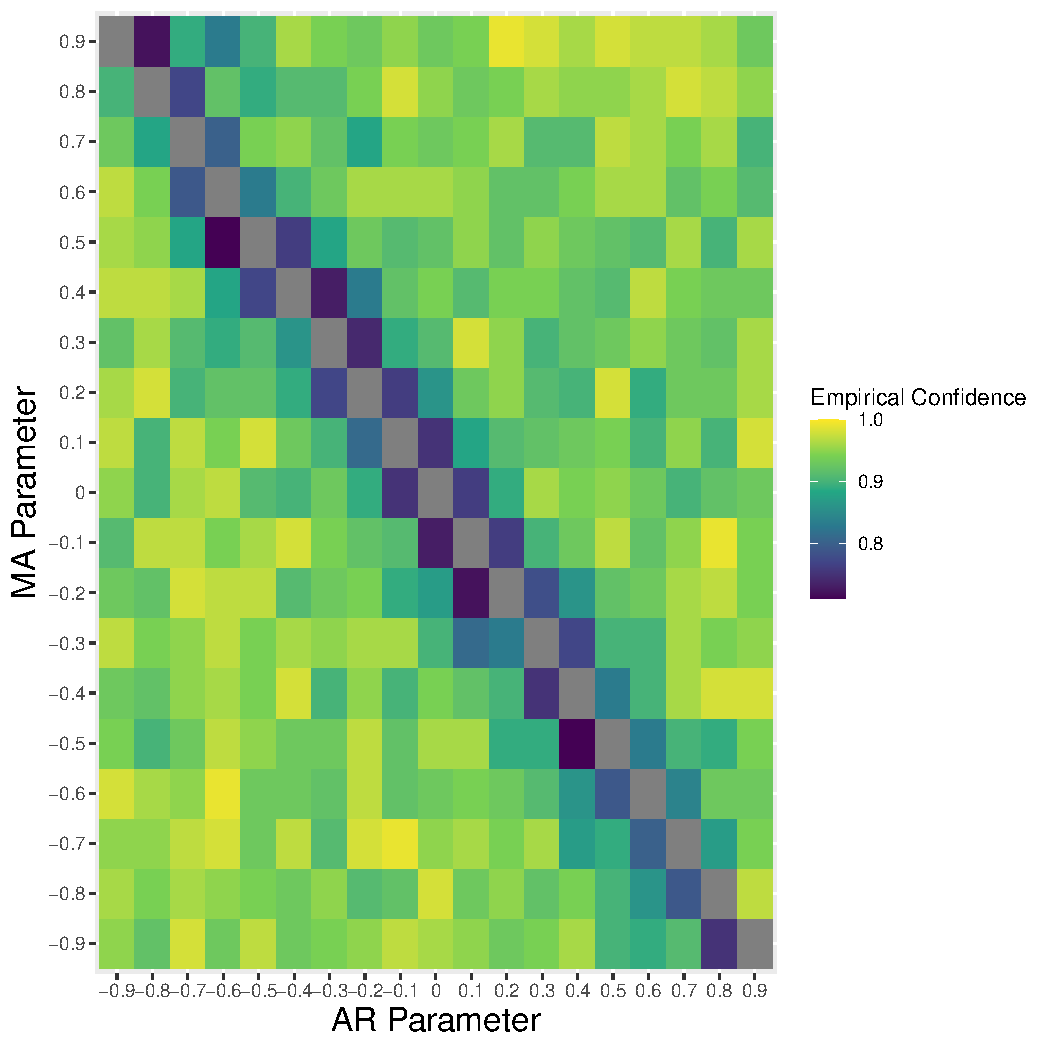
\includegraphics[width=\linewidth]{images/output/e_conf_o_3_2.pdf}
        \subcaption{$T = 1,000$}
    \end{subfigure}
    \hfill
    \begin{subfigure}{0.45\linewidth}
        \centering
        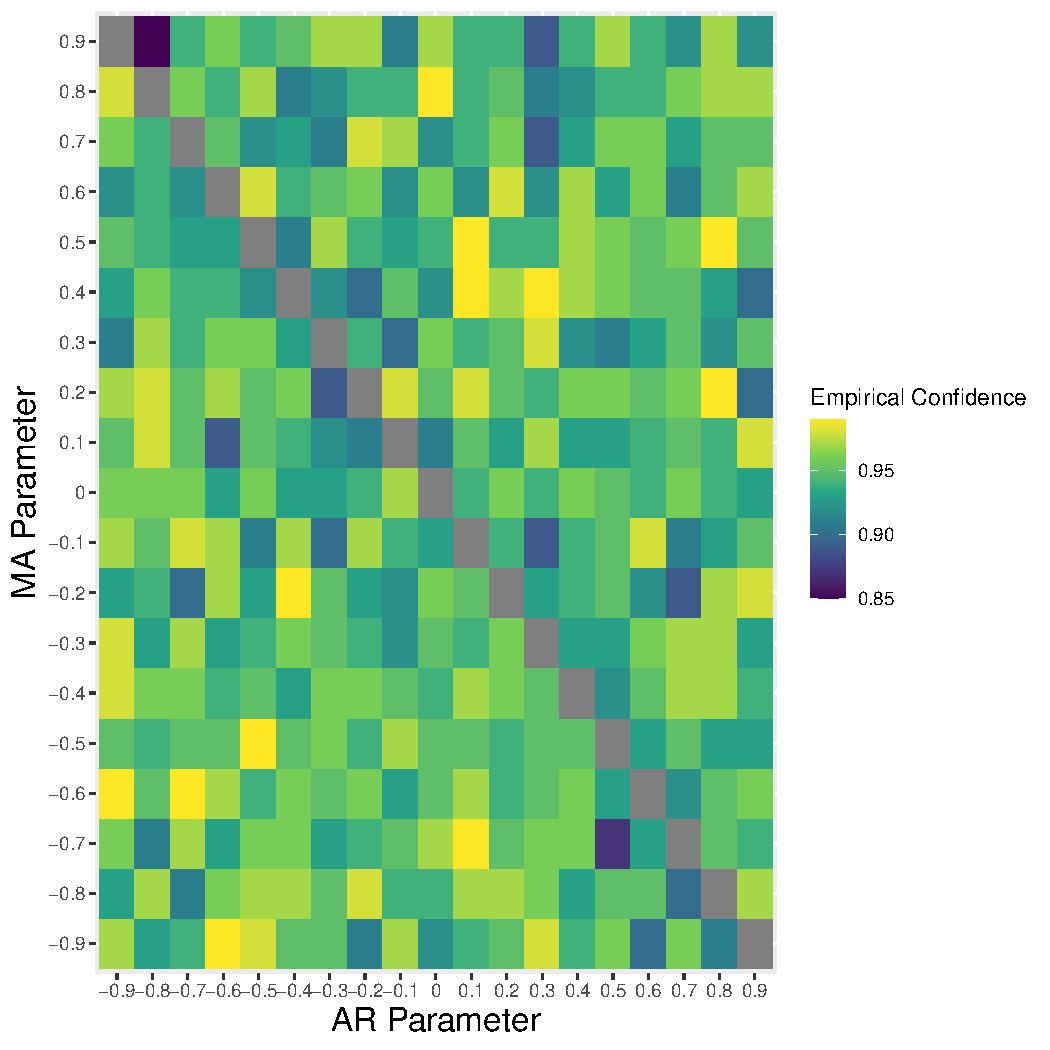
\includegraphics[width=\linewidth]{images/output/e_conf_o_4_2.pdf}
        \subcaption{$T = 10,000$}
    \end{subfigure}
    \caption{Rates at which point estimates for $\tau_o$ fall within confidence regions based on true values}
    \label{fig:e_conf_o}
\end{figure}
We begin with simulations of an ARMA(1,1)-Noise Model $\yy = X_t\uu + \bm{\varepsilon}$ parameterized by $\phi,\theta,\sigma_\eta^2,\sigma_\varepsilon^2$. Empirical confidence levels for each value-pair $(\phi,\theta)$ are based on a hundred simulations with $\sigma_\eta^2 = \sigma_\varepsilon^2 = 1,$ and $n_t = 2$. We first verify that the time series $ \mathbf{w}$ defined by $w_t = \bar{\yy}_{t\cdot}$, with MA parameter $\theta_b$ and innovation variance $\sigma_b^2$, produces time series estimates with normalized covariance close to $\Sigma_{\phi,\theta_b}$. For each set of parameters, we calculate the true values of $\theta_b$ and $\sigma_b^2$.  We then fit $(\hat{\phi},\hat{\theta}_b)$ with $\bar{\mathbf{w}}$ and construct confidence regions centered around those estimates, counting the rates at which these confidence regions capture the true parameter values. These empirical confidences are displayed in Figure \ref{fig:e_conf_o}. 



\begin{figure}[H]
\centering
    \begin{subfigure}{0.45\linewidth}
        \centering
        
\includegraphics[width=\linewidth]{images/output/e_conf_l_3_2.pdf}
        \subcaption{$T = 1000$}
    \end{subfigure}
    \hfill
    \begin{subfigure}{0.45\linewidth}
        \centering
        
\includegraphics[width=\linewidth]{images/output/e_conf_l_4_2.pdf}
        \subcaption{$T = 10,000$}
        
    \end{subfigure}
    \caption{Rates at which point estimates for $\tau_l$ fall within confidence regions based on sample estimates}
    \label{fig:e_conf_l}
\end{figure}

Confidence regions calculated with $\alpha = .05$ capture true values at rates close to the predicted confidence of $95\%$. As we are ultimately interested in estimating the parameters $\phi, \theta, \sigma_\eta^2$, we now see how well confidence regions based on applying the Delta Method to $\Sigma_{o}$ perform. The results in Figure \ref{fig:e_conf_l} were generated by simulating realizations of an ARMA(1,1)-Noise, estimating time series parameters $\phi$ and $\theta$, then using the Delta Method to construct $95\%$ confidence intervals.  





For both observable and latent parameters we can see performance dipped for parameter combinations $(\phi,\theta)$ close to the $\phi + \theta = 0$ line for time series of length $T = 1000$. However, we can see that performance improved for $T=10,000$, suggesting that parameter estimates for ARMA(1,1) processes that resemble white noise take longer to converge to their asymptotic distributions.


\section{REMARCS Model Fitting}
% \input{images/output/fearma_l1_conf.txt}
% \input{images/output/fearma_l2_conf.txt}


In order to assess the efficacy of this method, simulations were conducted with varying combinations of ARMA parameters $(\phi,\theta)$. In Figure \ref{fig:conf_heatmap}, we can see the proportion of 100 simulations that yielded confidence regions successfully capturing $\beta = (43,-0.001,0.25)$ (left) and $(\phi,\theta,\sigma_\eta^2)$ (right). One observation we can make is that the estimation of time series parameters appears to be hindered close to the line defined by $\phi + \theta = 0$. This under-performance is mitigated as $T$ grows, indicating that time series more closely resembling white noise will require larger values of $T$ for accurate estimation. 
\begin{figure}[H]
    \centering

    \begin{subfigure}{0.48\textwidth}
        \centering
        
\includegraphics[width=\linewidth]{images/output/l1_conf.pdf}
        \caption{Fixed Effect Parameter Estimation}
        \label{fig:sub1}
    \end{subfigure}
    \hfill
    \begin{subfigure}{0.48\textwidth}
        \centering
        
\includegraphics[width=\linewidth]{images/output/l2_conf.pdf}
        \caption{Time Series Parameter Estimation}
        \label{fig:sub2}
    \end{subfigure}
    \caption{Empirical confidences with which model parameters fall within confidence regions generated after model convergence}
    \label{fig:conf_heatmap}
\end{figure}

\subsection{Development of model parameter estimates}
Now that we've seen some aggregate results displaying the efficacy of this method under different parameters, we highlight some individual realizations of specific parameter combinations and observe how the parameter estimates evolve as the algorithm progresses. 
\subsubsection{Case: $\uu$ and $\mathbf{w}$ are ARMA(1,1)}
We start with a single simulation of the most general case of our model, one in which all parameters are nonzero. Exact values are given below:  
\begin{table}[H]
\centering\begin{tabular}{lccccccccc}
\hline
$T$ & sims & $\phi$ & $\theta$ & $\sigma_\eta^2$ & $\sigma_\varepsilon^2$ & $\beta_0$ & $\beta_1$ & $\beta_2$ \\
1000 & 1 & 0.9 & -0.6 & 1 & 10 & 40 & -0.001 & 2 \\
\hline
\end{tabular}
\caption{Parameter values for simulated REMARCS model with all nonzero parameters}
\label{tab:param_estimates}
\end{table}



We begin by displaying the individual data, along with the eventual fitted values.

\begin{figure}[H]
    \centering
    % Row 1
    \begin{subfigure}{0.45\textwidth}
        \centering
        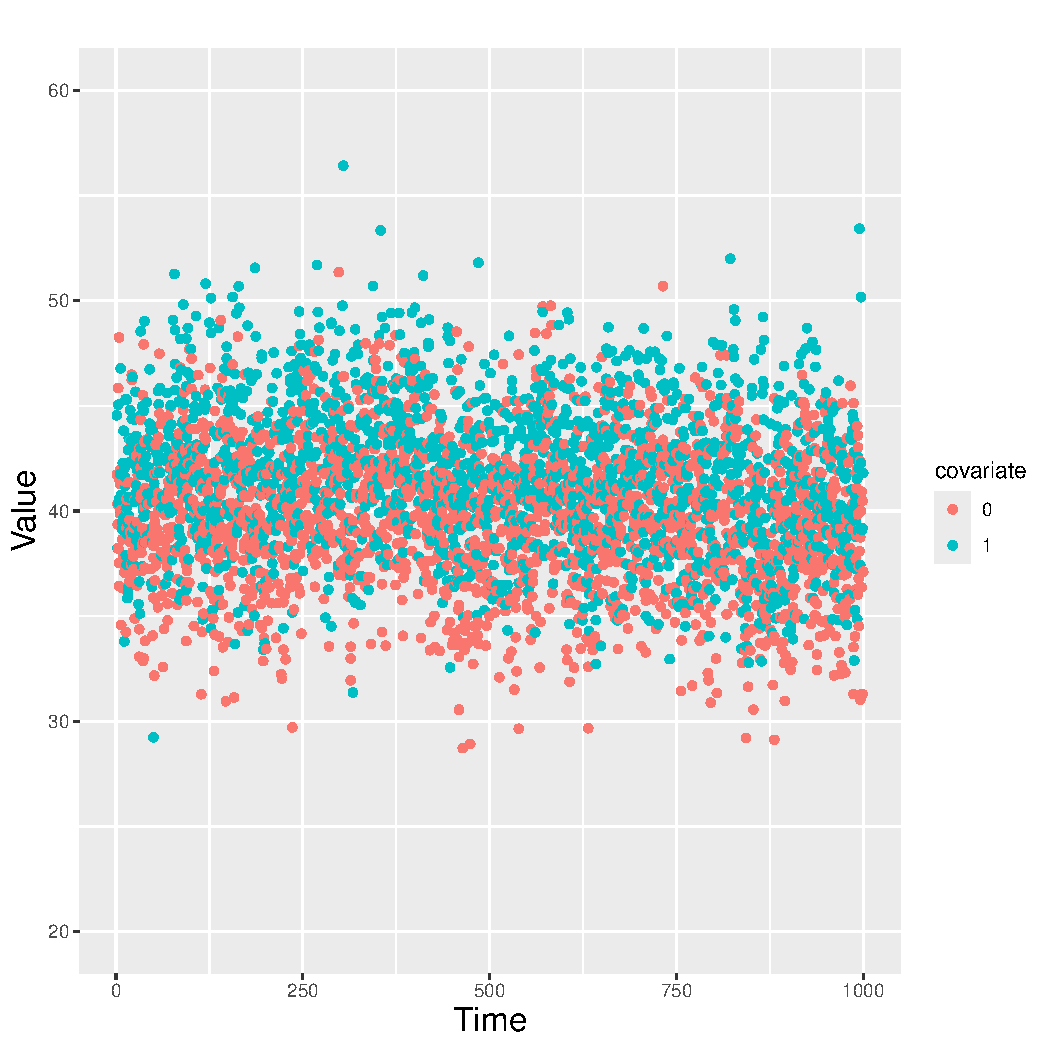
\includegraphics[width=\linewidth]{images/output/sim_arma_full.pdf}
        \caption{Observed Data}
    \end{subfigure}
    \hfill
    \begin{subfigure}{0.45\textwidth}
        \centering
        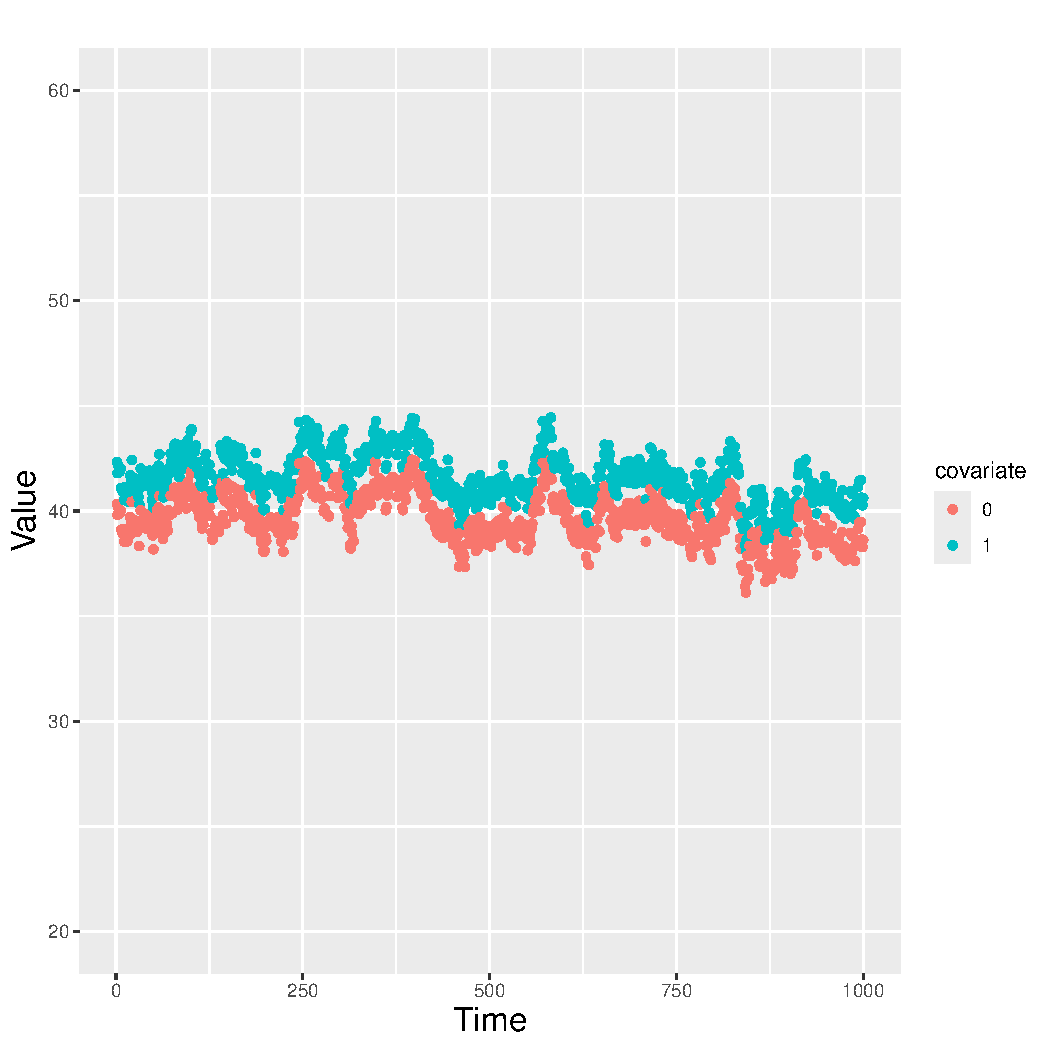
\includegraphics[width=\linewidth]{images/output/sim_arma_fitted.pdf}
        \caption{Fitted Values}
    \end{subfigure}

    \caption{A realization of a REMARCS model before and after fitting}
    \label{fig:single_sim}
\end{figure}

% \begin{figure}[H]
%     \centering
%     % Row 1
%     \begin{subfigure}{0.45\textwidth}
%         \centering
%         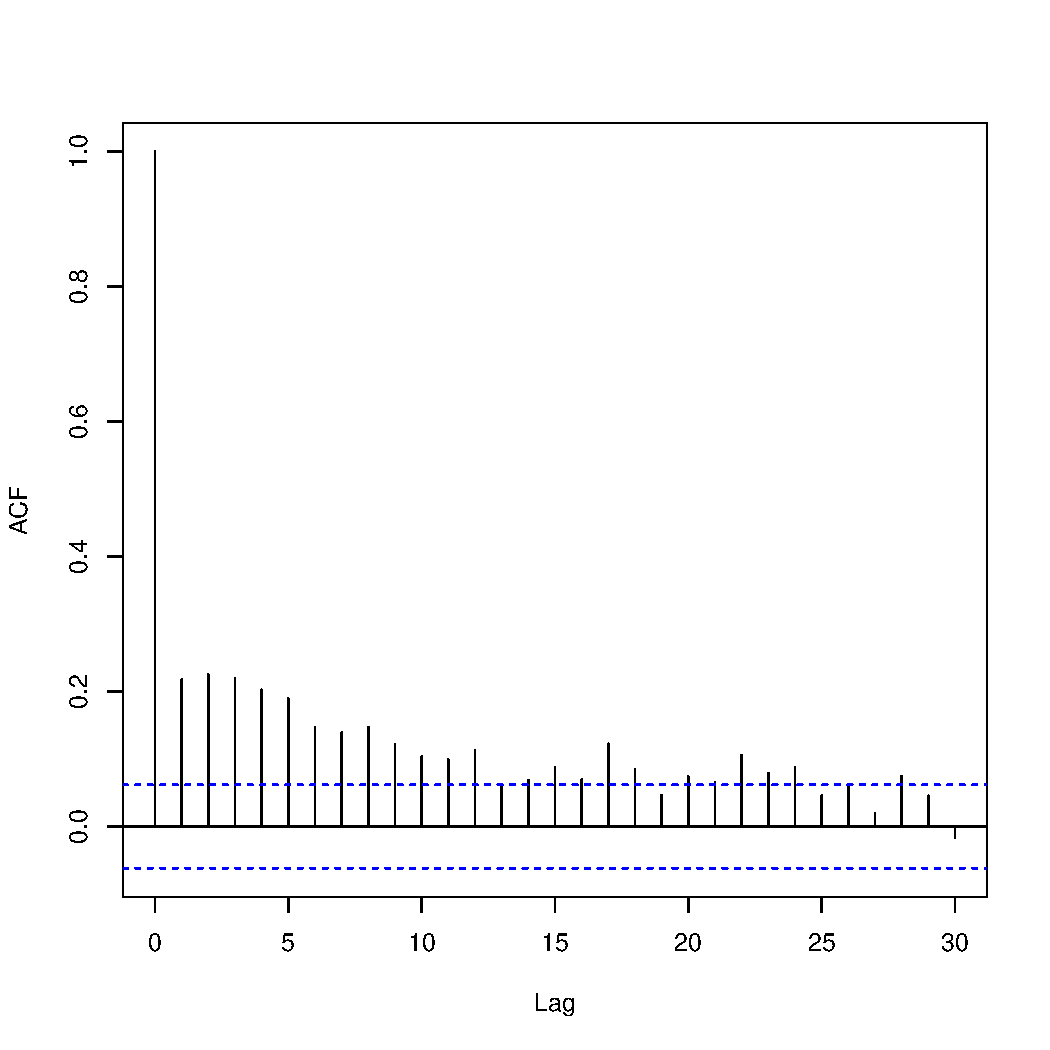
\includegraphics[width=\linewidth,page=1]{images/output/sim_arma_acfs.pdf}
%         \caption{SACF of Initial Residual Aggregates}
%     \end{subfigure}
%     \hfill
%     \begin{subfigure}{0.45\textwidth}
%         \centering
%         \includegraphics[width=\linewidth, page=2]{images/output/sim_arma_acfs.pdf}
%         \caption{SACF of Final Residual Aggregates}
%     \end{subfigure}
%     \caption{Temporal correlation in aggregated residuals before and after model convergence}
%     \label{fig:sim_arma_acfs}
% \end{figure}

% \textcolor{blue}{Display standard errors alongside fixed effect estimates}

Once the convergence criterion of $|l(\hat{\xi}^{(k+1)})-l(\hat{\xi}^{(k)})|<.001 $ is satisfied, we take a look at the significance of ``observable'' time series parameter estimates $(\hat{\phi},\hat{\theta}_b)$. Seeing that both $\hat{\phi}$ and $\hat{\theta}_b$ are significant in the left panel of Figure \ref{fig:single_sim_inf_arma}, we proceed to fit estimates for $\theta$ and $\sigma_\eta^2$ using $H$ in Equation \ref{eq:H_arman}. The right panel of the same figure shows the resulting confidence region after applying the Delta Method, and we can see that the true parameters are successfully captured.

\begin{figure}[H]
    \centering
    \begin{subfigure}{0.48\textwidth}
        \centering
        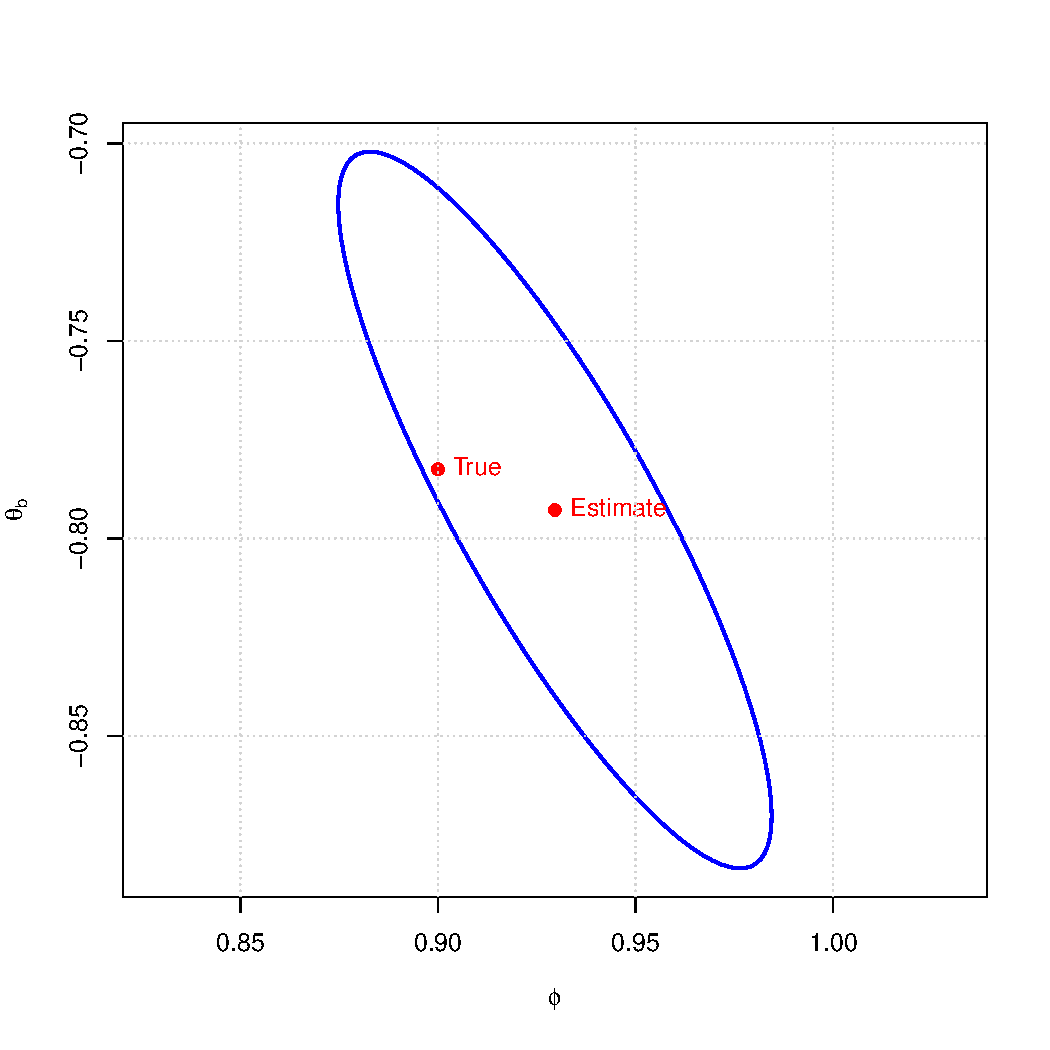
\includegraphics[width=\linewidth]{images/output/single_sim_observed.pdf}
        \caption{Confidence region for ARMA parameters of $\mathbf{w}$}
    \end{subfigure}
    \hfill
    \begin{subfigure}{0.48\textwidth}
        \centering
        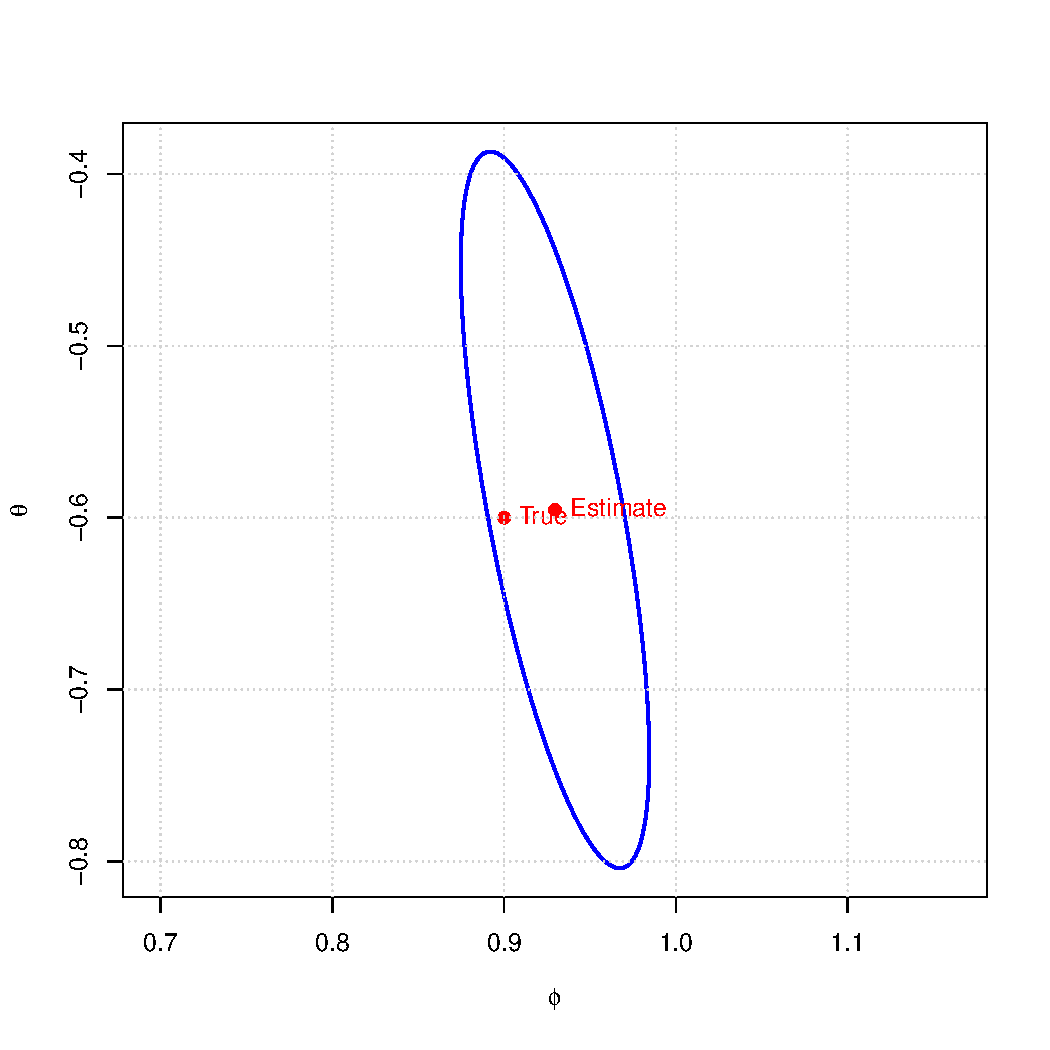
\includegraphics[width=\linewidth]{images/output/single_sim_latent.pdf}
        \caption{Confidence region for ARMA parameters of $\mathbf{u}$}
    \end{subfigure}
    \caption{Confidence regions for time series parameter estimates of latent ARMA(1,1) process}
    \label{fig:single_sim_inf_arma}
\end{figure}


In the table below we can see how properly accounting for temporal correlation helps update parameter estimates:


\begin{table}[H]
\centering\begin{tabular}{lccccccc}
\toprule
Parameter & $\beta_0$ & $\beta_1$ & $\beta_2$ & $\sigma_\varepsilon^2$ & $\phi$ & $\theta$ & $\sigma_\eta^2$ \\
\midrule
True Value & 40.0000 & -0.0010 & 2.0000 & 10.0000 & 0.9000 & -0.6000 & 1.0000 \\
\midrule
Initial estimate & 40.4306 & -0.0016 & 1.9526 & 11.5826 & 0.0000 & 0.0000 & 0.0000 \\
Final estimate & 40.4352 & -0.0017 & 1.9857 & 9.8552 & 0.9296 & -0.5955 & 0.9482 \\
\hline
\end{tabular}
\caption{Parameter estimates for REMARCS model with all nonzero parameters, before and after convergence}
\label{tab:param_estimates}
\end{table}


\subsubsection{Case: $\uu$ is AR(1)}
We now look at data simulated from a restricted model with the following parameters: 
\begin{table}[H]
\centering\begin{tabular}{lccccccccc}
\hline
$T$ & sims & $\phi$ & $\theta$ & $\sigma_\eta^2$ & $\sigma_\varepsilon^2$ & $\beta_0$ & $\beta_1$ & $\beta_2$ \\
1000 & 1 & 0.8 & 0 & 10 & 10 & -10 & 0.001 & 1 \\
\hline
\end{tabular}
\caption{Parameter values for simulated REMARCS model with a latent AR(1) process}
\label{tab:param_values_ma}
\end{table}


\begin{figure}[H]
    \centering
    \begin{subfigure}{0.48\textwidth}
        \centering
        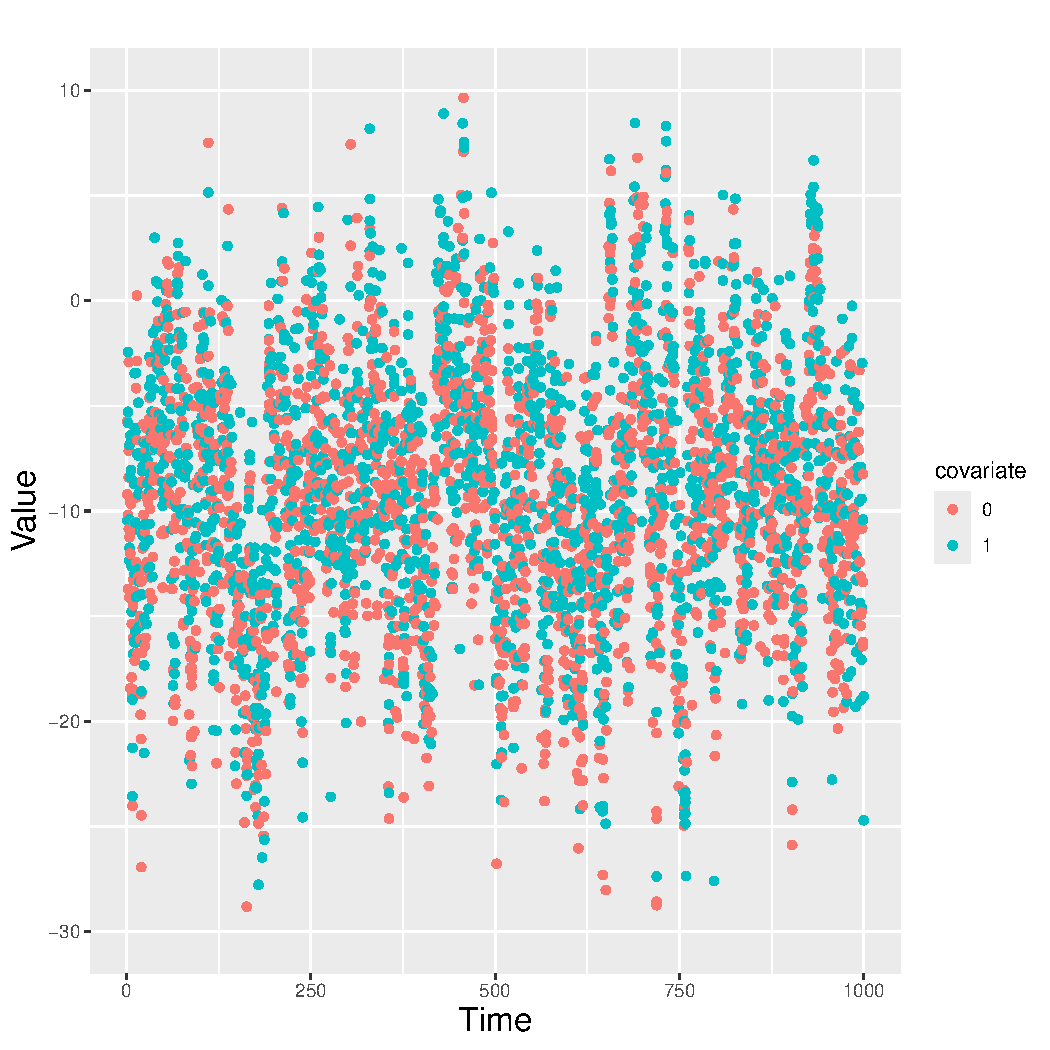
\includegraphics[width=\linewidth]{images/output/sim_ma_full.pdf}
        \caption{Observations}
    \end{subfigure}
    \hfill
    \begin{subfigure}{0.48\textwidth}
        \centering
        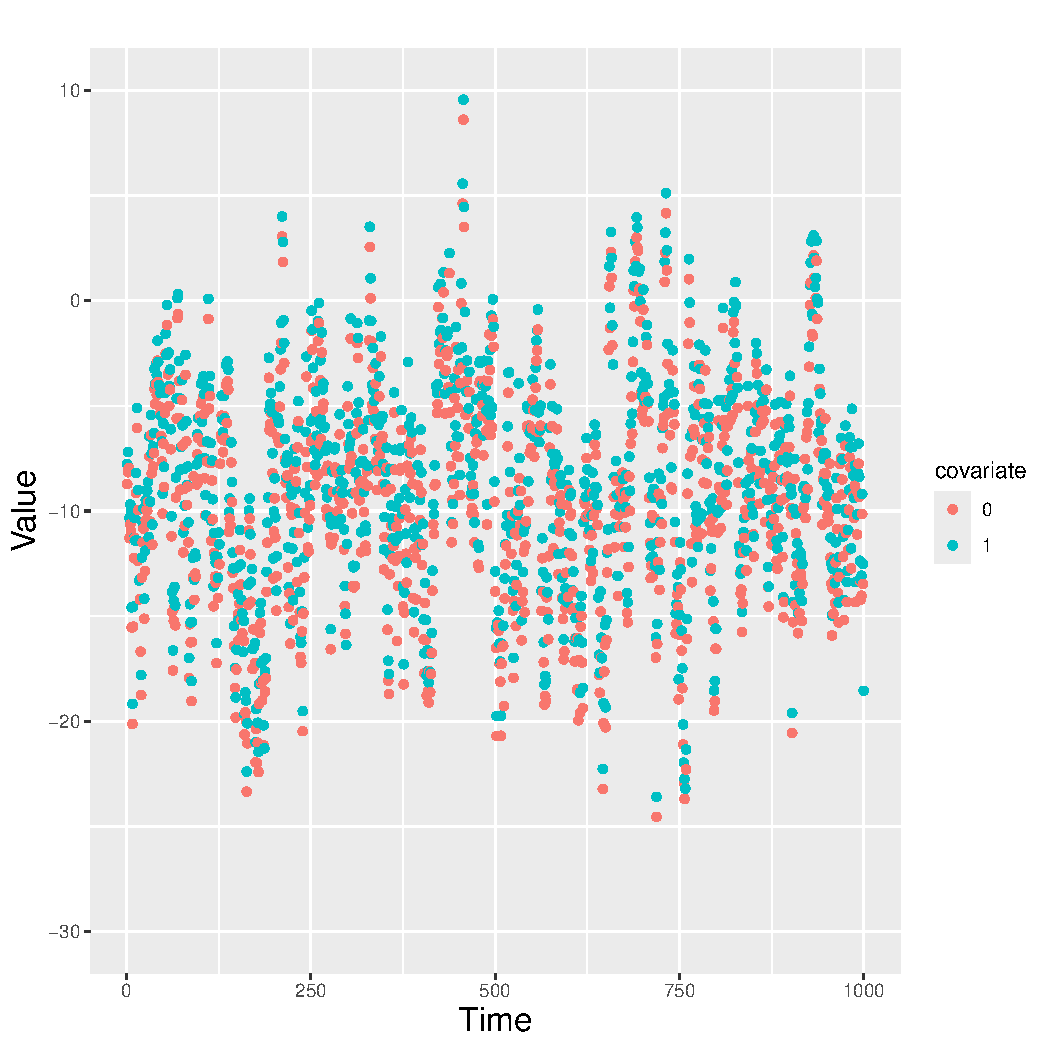
\includegraphics[width=\linewidth]{images/output/sim_ma_fitted.pdf}
        \caption{Fitted Values}
    \end{subfigure}
    \caption{Observations and fitted values from a REMARCS model with a latent AR(1) time series}
    \label{fig:single_sim_ma}
\end{figure}

% \begin{figure}[H]
%     \centering
%     % Row 1
%     \begin{subfigure}{0.45\textwidth}
%         \centering
%         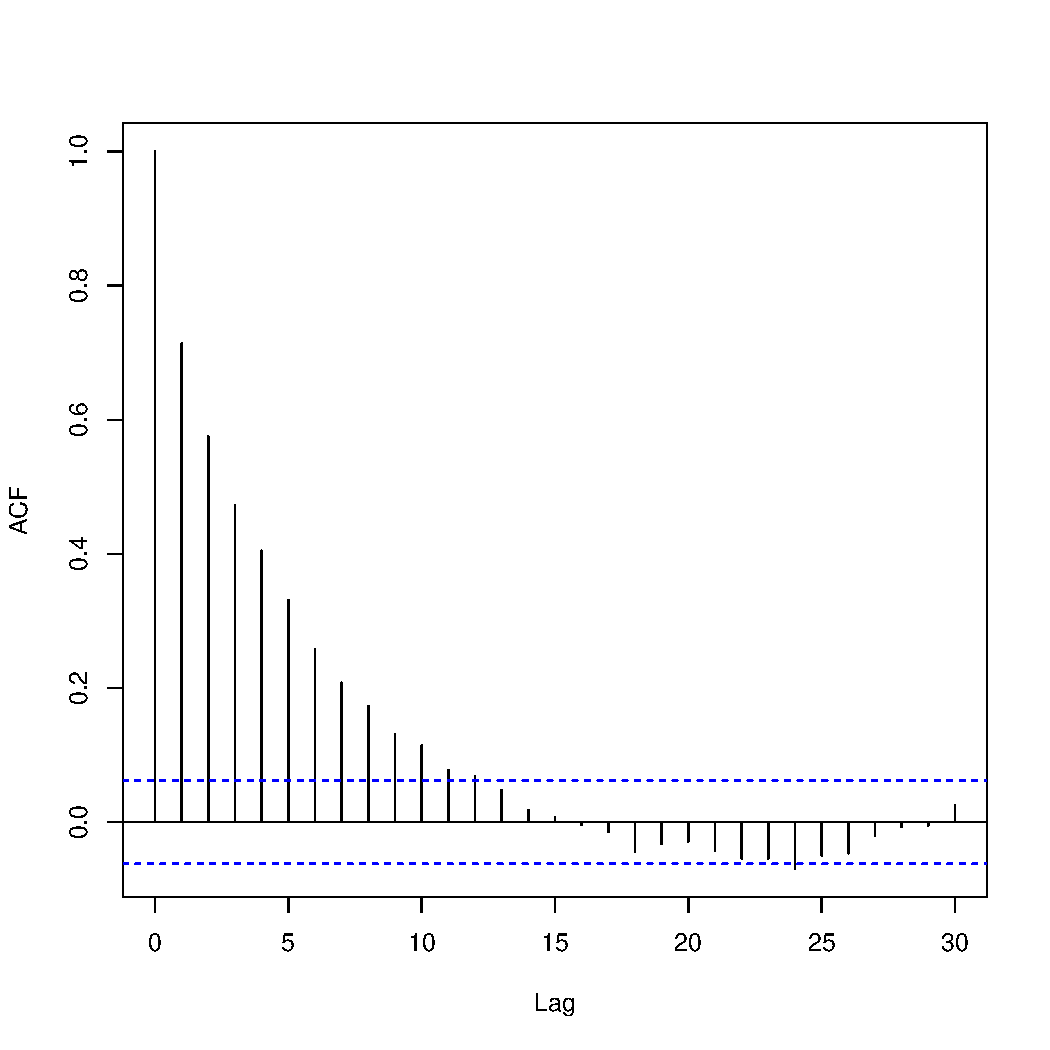
\includegraphics[width=\linewidth,page=1]{images/output/sim_ma_acfs.pdf}
%         \caption{SACF of Initial Residual Aggregates}
%     \end{subfigure}
%     \hfill
%     \begin{subfigure}{0.45\textwidth}
%         \centering
%         \includegraphics[width=\linewidth, page=2]{images/output/sim_ma_acfs.pdf}
%         \caption{SACF of Final Residual Aggregates}
%     \end{subfigure}
%     \caption{Temporal correlation in aggregated residuals before and after model convergence}
%     \label{fig:sim_ma_acfs}
% \end{figure}
\begin{table}[H]
\centering\begin{tabular}{lccccccc}
\toprule
Parameter & $\beta_0$ & $\beta_1$ & $\beta_2$ & $\sigma_\varepsilon^2$ & $\phi$ & $\theta$ & $\sigma_\eta^2$ \\
\midrule
True Value & -10.0000 & 0.0010 & 1.0000 & 10.0000 & 0.8000 & 0.0000 & 10.0000 \\
\midrule
Initial estimate & -10.2365 & 0.0011 & 1.1015 & 38.6200 & 0.0000 & 0.0000 & 0.0000 \\
Final estimate & -10.0172 & 0.0007 & 0.9519 & 9.8354 & 0.8130 & -0.0673 & 10.7934 \\
\hline
\end{tabular}
\caption{Parameter estimates REMARCS model with latent AR(1) Time Series, before and after convergence  }
\label{tab:param_estimates_ma}
\end{table}



After having applied the general method to observations and the convergence of parameter estimates, we now perform inference on $(\hat{\phi}, \hat{\theta}_b)$. Seeing that both estimates are significant in the left side of Figure \ref{fig:single_sim_ma}, we proceed as before with the most general form of $H$. 

\begin{figure}[htbp]
    \centering
    \begin{subfigure}{0.48\textwidth}
        \centering
        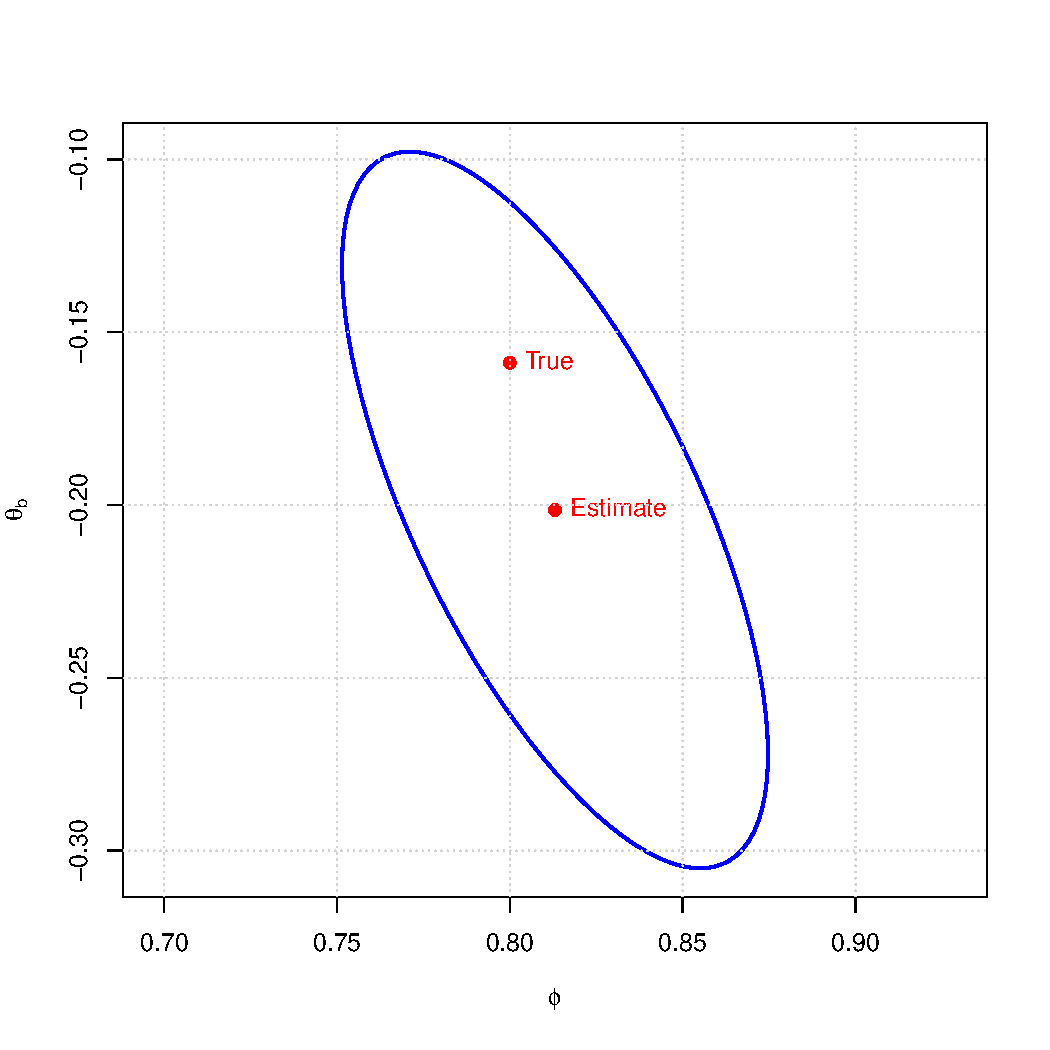
\includegraphics[width=\linewidth]{images/output/single_sim_ma_observed.pdf}
        \caption{Confidence Region for Parameters of $\mathbf{w}$}

    \end{subfigure}
    \hfill
    \begin{subfigure}{0.48\textwidth}
        \centering
        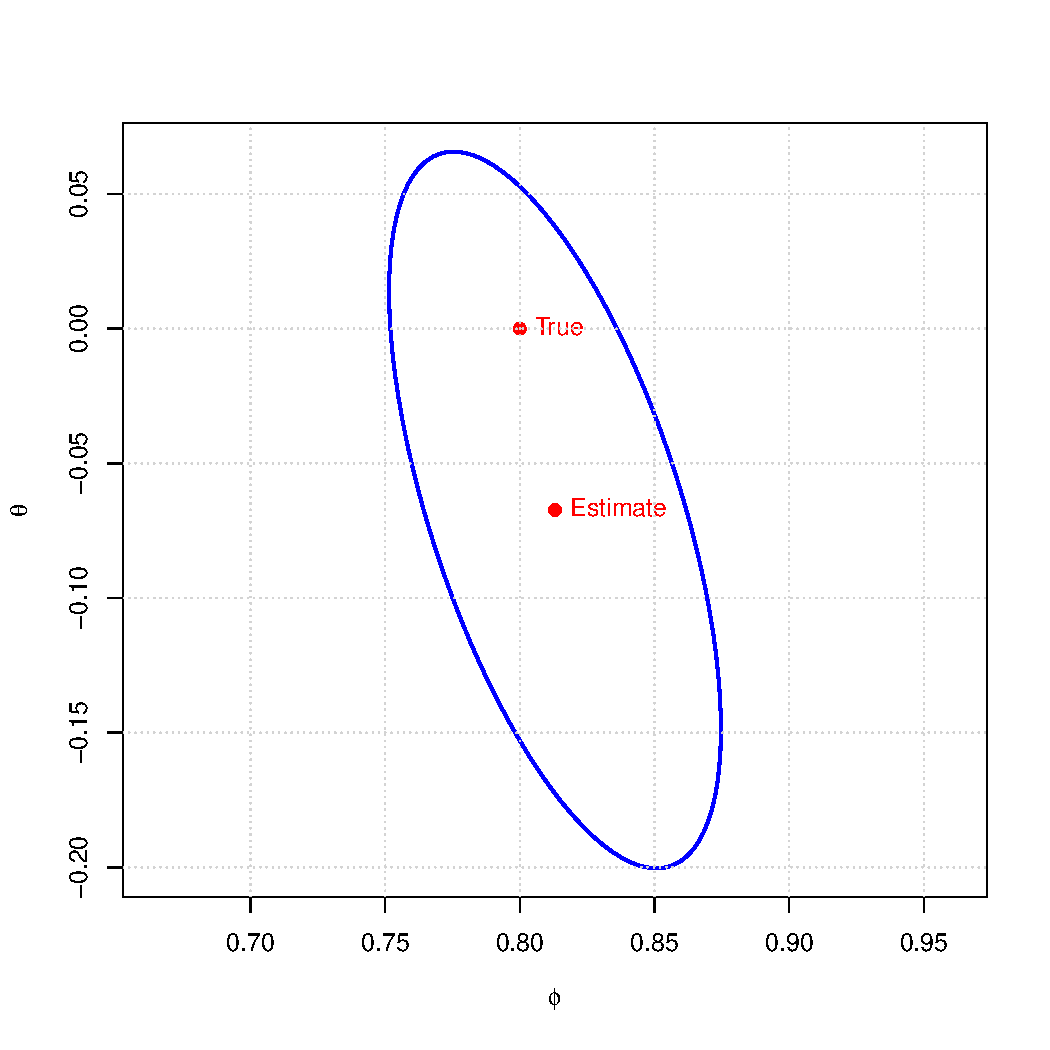
\includegraphics[width=\linewidth]{images/output/single_sim_ma_latent.pdf}
        \caption{Confidence Region for Parameters of $\mathbf{u}$}
    \end{subfigure}
    \caption{Confidence regions for time series parameter estimates of latent ARMA(1,1) process}
    \label{fig:single_sim_ma_inf}
\end{figure}


We then see in the right panel of Figure \ref{fig:single_sim_ma} that the resulting estimate for $\theta$ is insignificant, prompting us to repeat the estimation of $\sigma_\eta^2$ by using $H_\theta$ in Equation \ref{eq:H_theta}. While the standard error for $\hat{\phi}$ is unaffected, the restriction of $\hat{\theta}$ will affect $\widehat{\sigma_\eta^2}$. To complete this analysis, the algorithm would be restarted, now with the restriction $\hat{\theta} = 0$.

\begin{figure}[H]
    \centering
    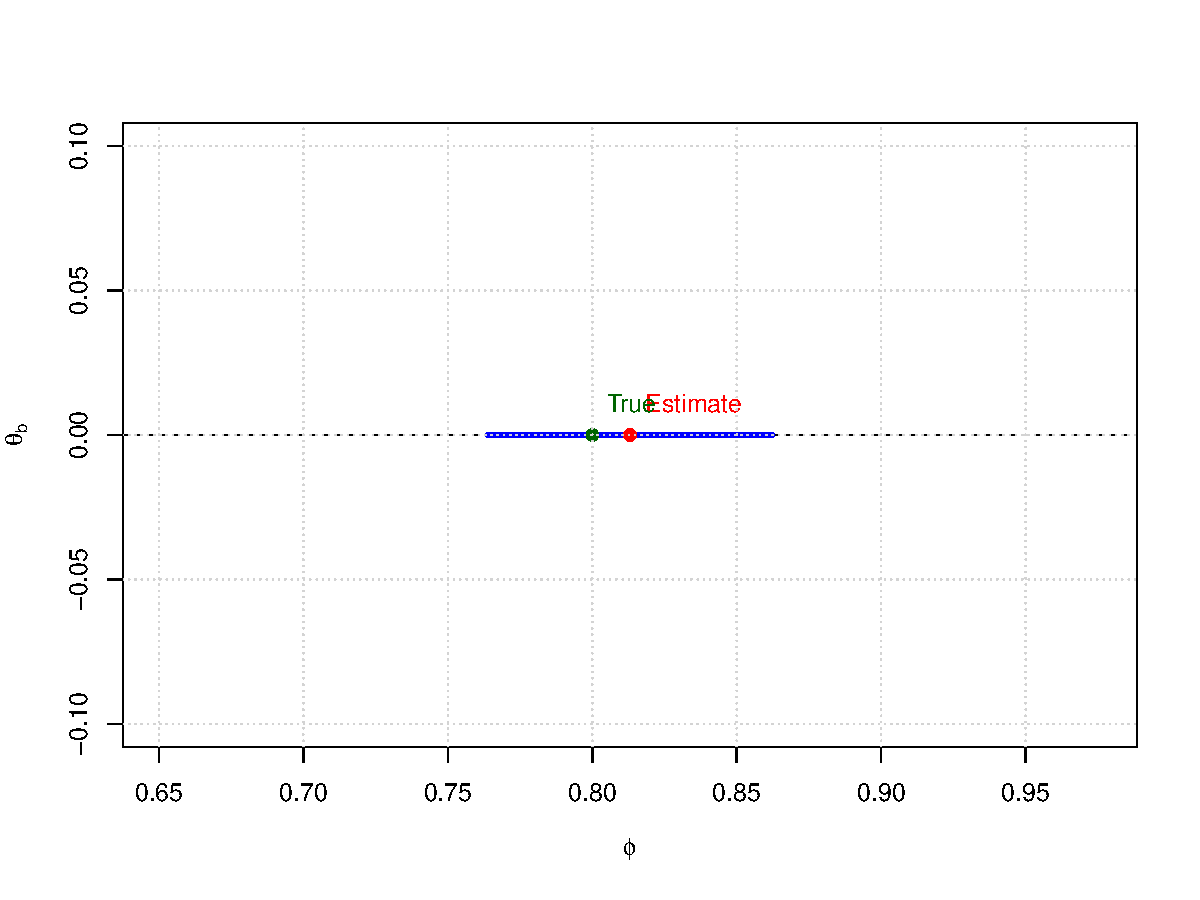
\includegraphics[width=0.5\linewidth]{images/output/single_sim_ma_restricted.pdf}
    \caption{Confidence interval for $\phi$ after restricting model}
    \label{fig:single_sim_ma_restricted}
\end{figure}


\subsubsection{Case: $\uu$ is MA(1)}

We now restrict $\phi = 0$ and simulate data with the following parameters:

\begin{table}[H]
\centering\begin{tabular}{lccccccccc}
\hline
$T$ & sims & $\phi$ & $\theta$ & $\sigma_\eta^2$ & $\sigma_\varepsilon^2$ & $\beta_0$ & $\beta_1$ & $\beta_2$ \\
1000 & 1 & 0 & 0.5 & 5 & 10 & -100 & 0.01 & 3 \\
\hline
\end{tabular}
\caption{Parameter values for simulated REMARCS model with a latent MA(1) process}
\label{tab:param_values_ar}
\end{table}



\begin{figure}[H]
    \centering
    % Row 1
    \begin{subfigure}{0.45\textwidth}
        \centering
        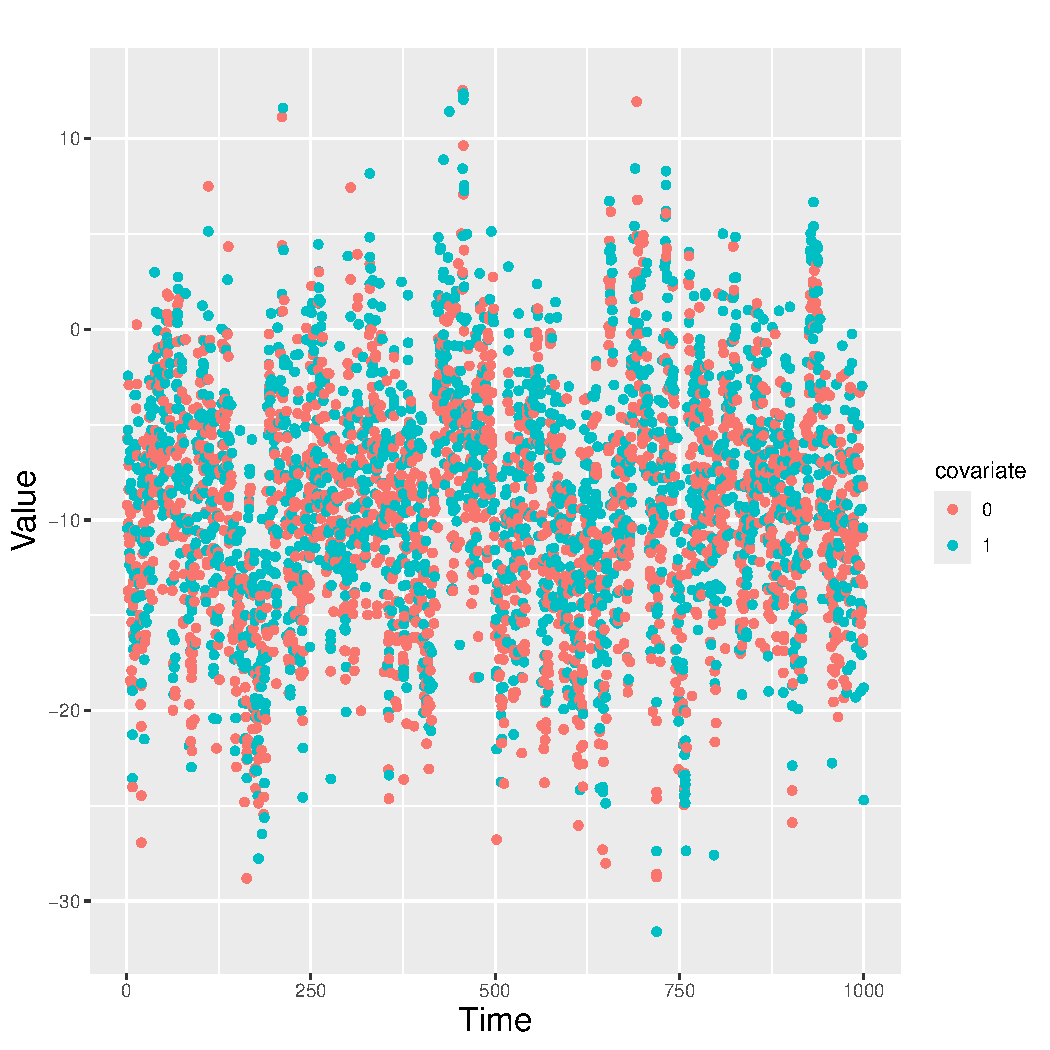
\includegraphics[width=\linewidth]{images/output/sim_ar_full.pdf}
        \caption{Realization}
    \end{subfigure}
    \hfill
    \begin{subfigure}{0.45\textwidth}
        \centering
        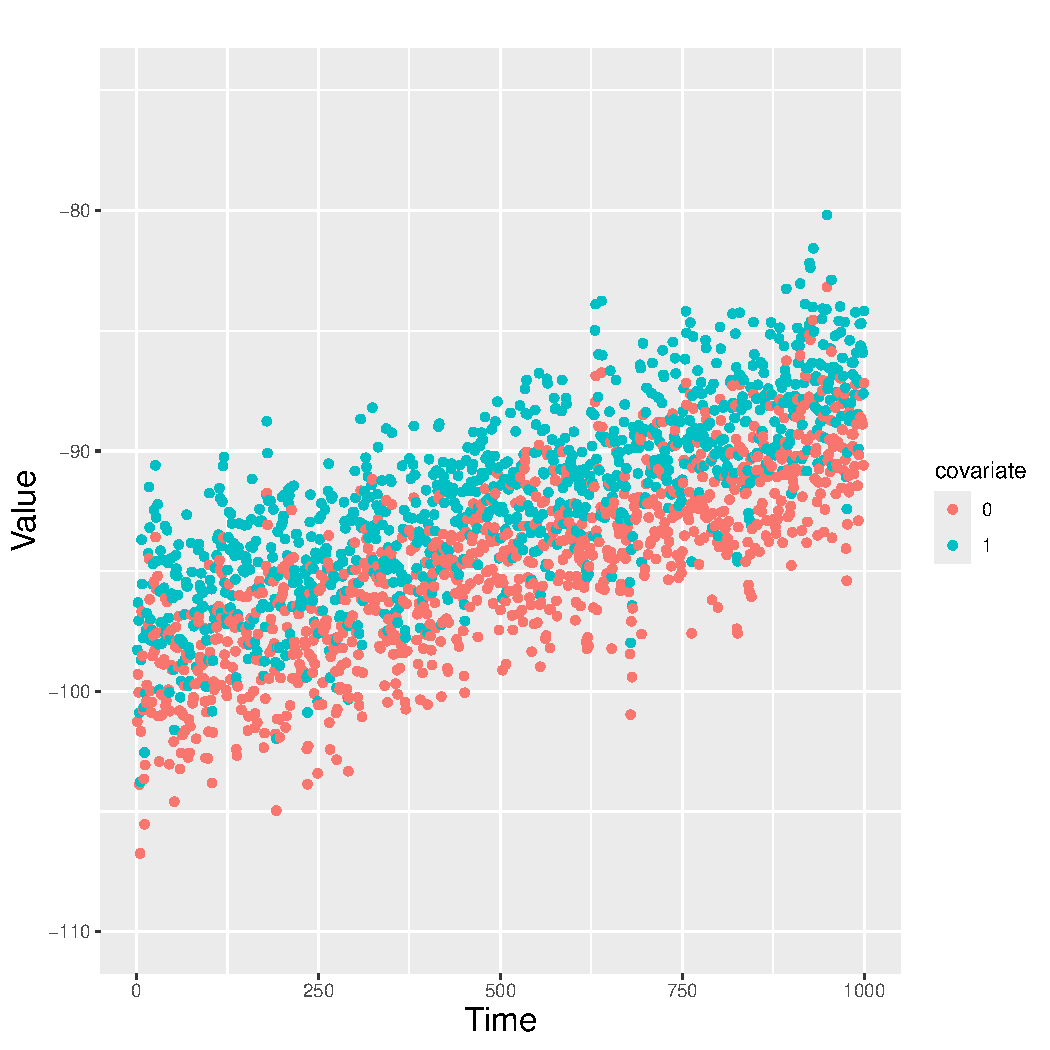
\includegraphics[width=\linewidth]{images/output/sim_ar_fitted.pdf}
        \caption{Fitted Model}
    \end{subfigure}
    \caption{Simulated REMARCS Model Before and After Fitting}
    \label{fig:single_sim_ar}
\end{figure}

% \begin{figure}[H]
%     \centering
%     % Row 1
%     \begin{subfigure}{0.45\textwidth}
%         \centering
%         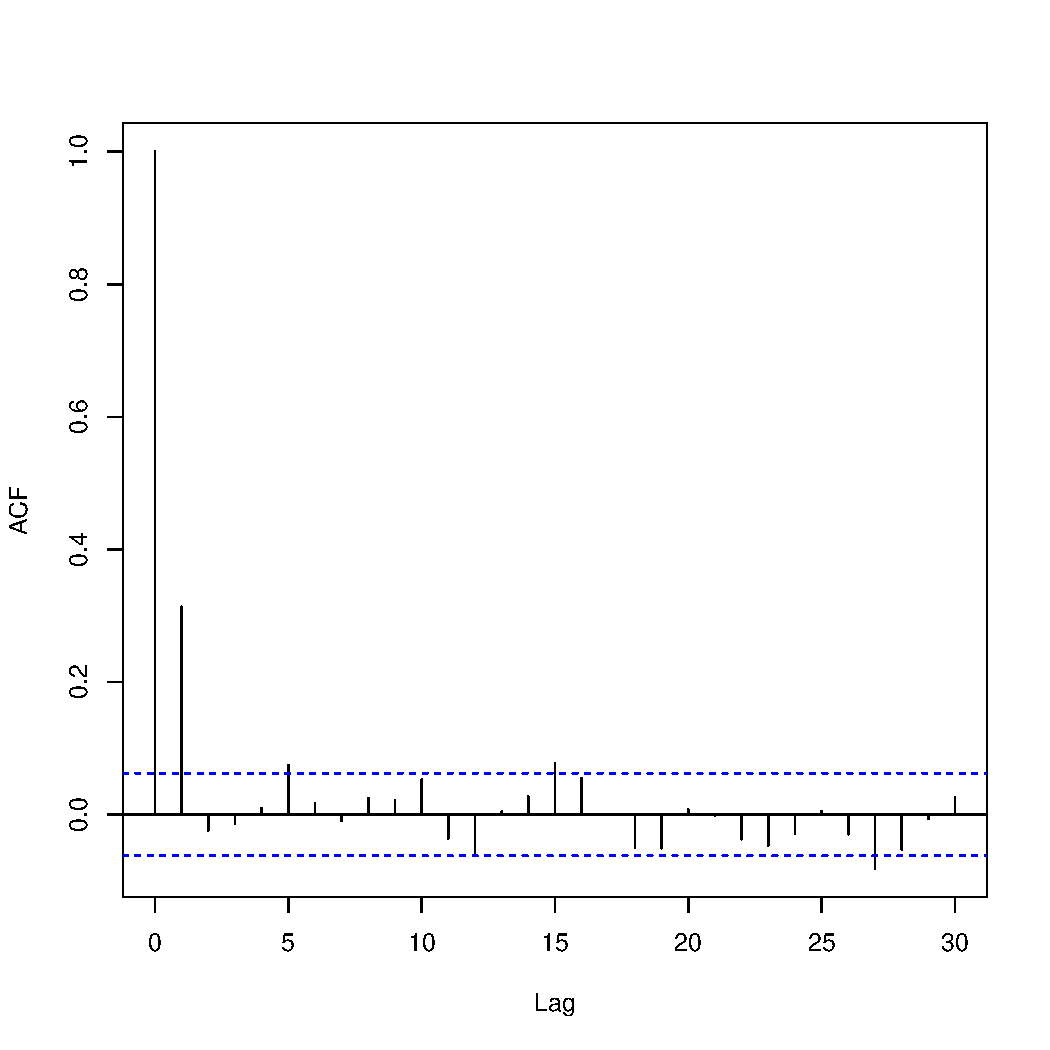
\includegraphics[width=\linewidth,page=1]{images/output/sim_ar_acfs.pdf}
%         \caption{SACF of Initial Residual Aggregates}
%     \end{subfigure}
%     \hfill
%     \begin{subfigure}{0.45\textwidth}
%         \centering
%         \includegraphics[width=\linewidth, page=2]{images/output/sim_ar_acfs.pdf}
%         \caption{SACF of Final Residual Aggregates}
%     \end{subfigure}
%     \caption{Temporal correlation in aggregated residuals before and after model convergence}
%     \label{fig:sim_ar_acfs}
% \end{figure}




We then initiate the algorithm as usual and obtain the following parameter estimates:
\begin{table}[H]
\centering\begin{tabular}{lccccccc}
\toprule
Parameter & $\beta_0$ & $\beta_1$ & $\beta_2$ & $\sigma_\varepsilon^2$ & $\phi$ & $\theta$ & $\sigma_\eta^2$ \\
\midrule
True Value & -100.0000 & 0.0100 & 3.0000 & 10.0000 & 0.0000 & 0.5000 & 5.0000 \\
\midrule
Initial estimate & -100.0109 & 0.0103 & 2.9861 & 16.5249 & 0.0000 & 0.0000 & 0.0000 \\
Final estimate & -100.0670 & 0.0104 & 2.9861 & 9.9510 & -0.0816 & 0.5900 & 5.1878 \\
\hline
\end{tabular}
\caption{Parameter estimates for REMARCS model with latent MA(1) time series, before and after convergence}
\label{tab:param_estimates_ar}
\end{table}



We take the final time series parameter estimates and perform inference on $\hat{\phi}$ and $\hat{\theta}_b$:
\begin{figure}[H]
    \centering

    % Row 1
    \begin{subfigure}{0.45\textwidth}
        \centering
        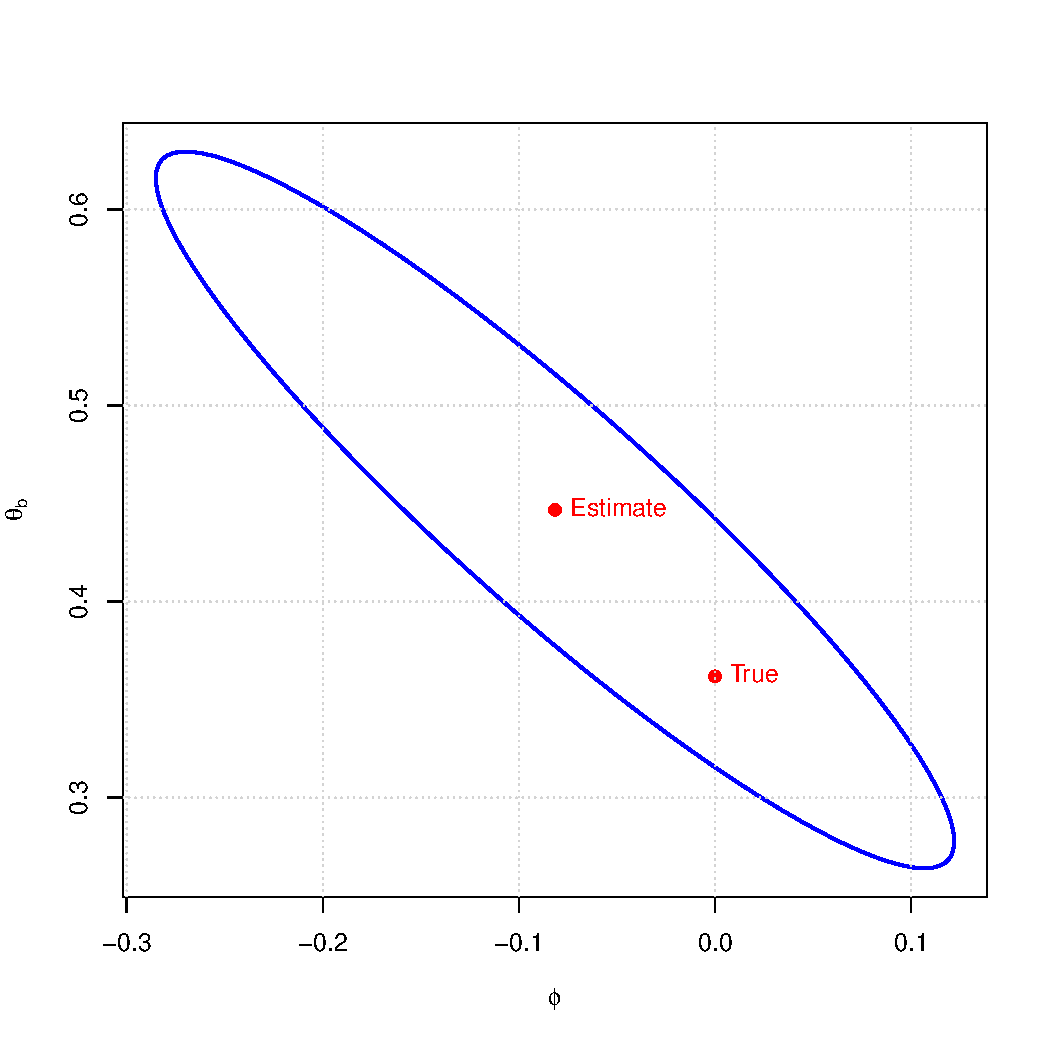
\includegraphics[width=\linewidth]{images/output/single_sim_ar_observed.pdf}
        \caption{Confidence region for $(\phi,\theta_b)$}
    \end{subfigure}
    \hfill
    \begin{subfigure}{0.45\textwidth}
        \centering
        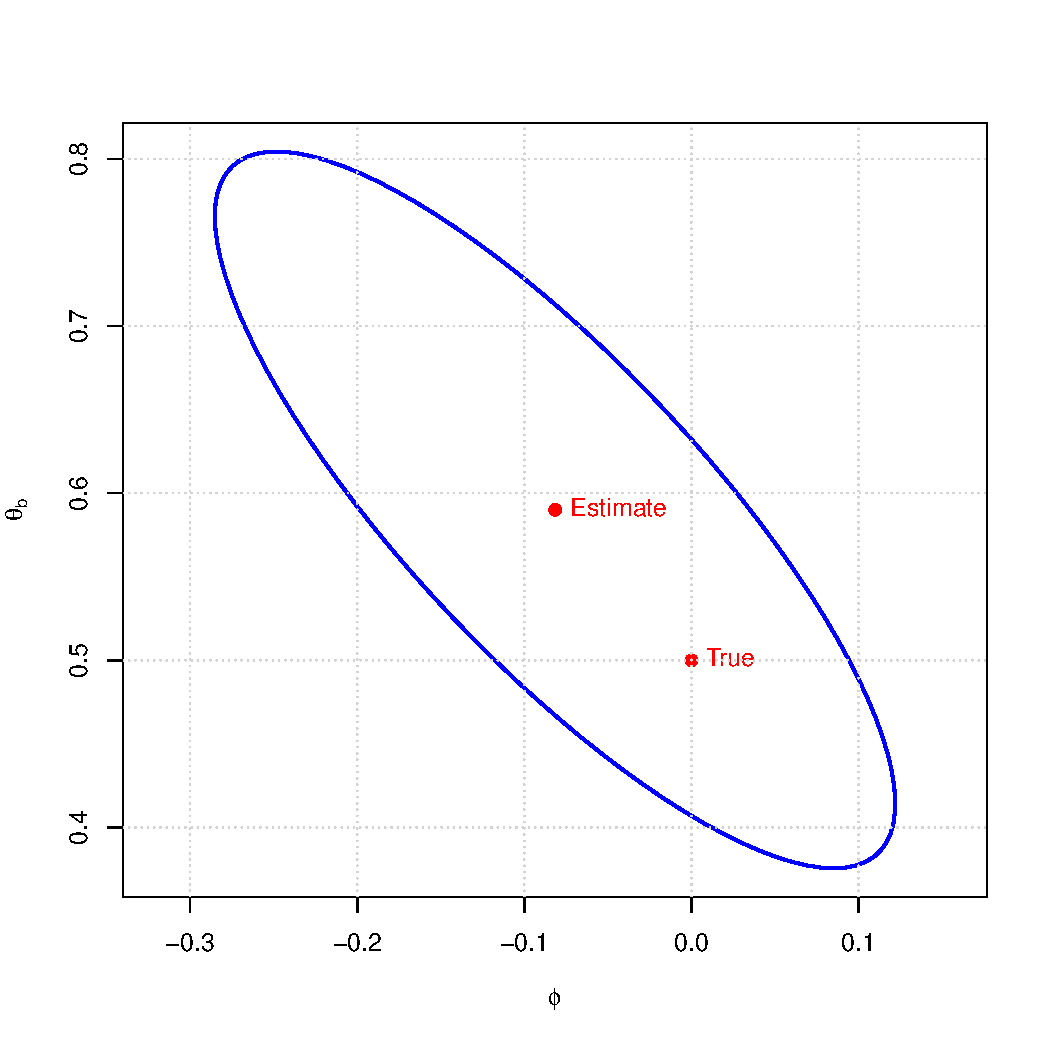
\includegraphics[width=\linewidth]{images/output/single_sim_ar_latent.pdf}
        \caption{Confidence region for $(\phi,\theta)$}
    \end{subfigure}

    % \vspace{0.5em}

    % % Row 2
    % \begin{subfigure}{0.45\textwidth}
    %     \centering
    %     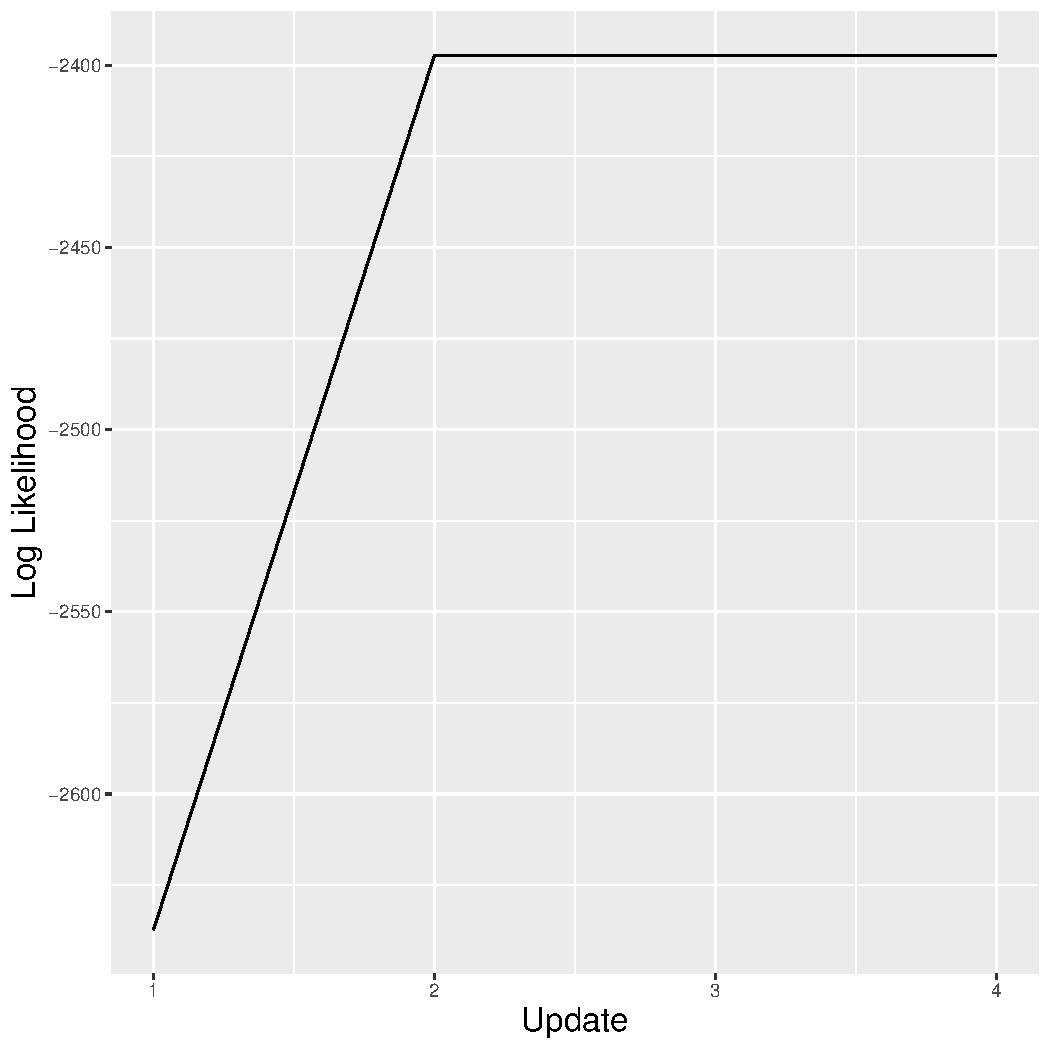
\includegraphics[width=\linewidth]{images/output/sim_ma_l2.pdf}
    %     \caption{Caption 3}
    % \end{subfigure}
    % \hfill
    % \begin{subfigure}{0.45\textwidth}
    %     \centering
    %     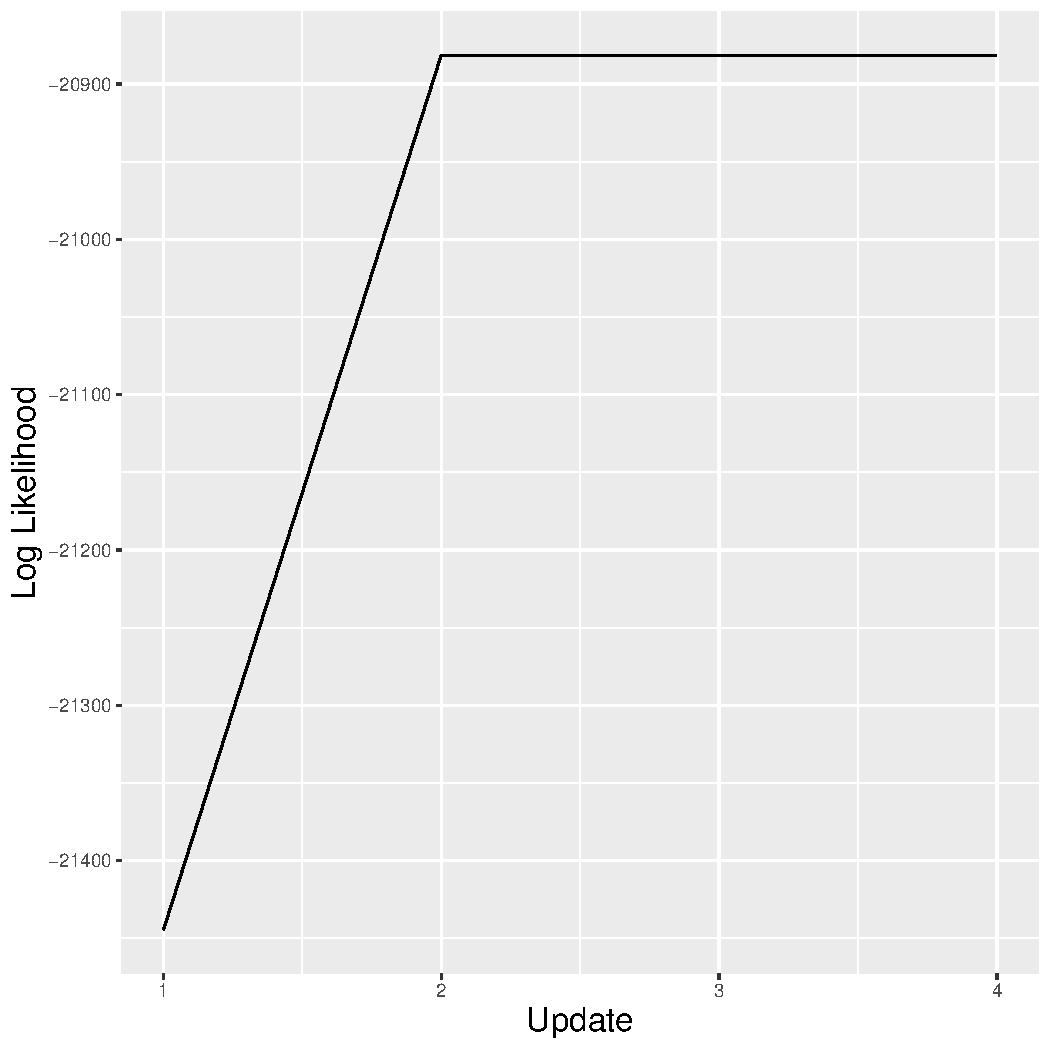
\includegraphics[width=\linewidth]{images/output/sim_ma_l.pdf}
    %     \caption{Caption 4}
    % \end{subfigure}

    \caption{Confidence regions for observable and latent moving average parameters before restricting REMARCS model with $\theta_b = 0$ }
    \label{fig:single_sim_ar_unrestricted}
\end{figure}

\begin{figure}[H]
    \centering

    % Row 1
    \begin{subfigure}{0.45\textwidth}
        \centering
        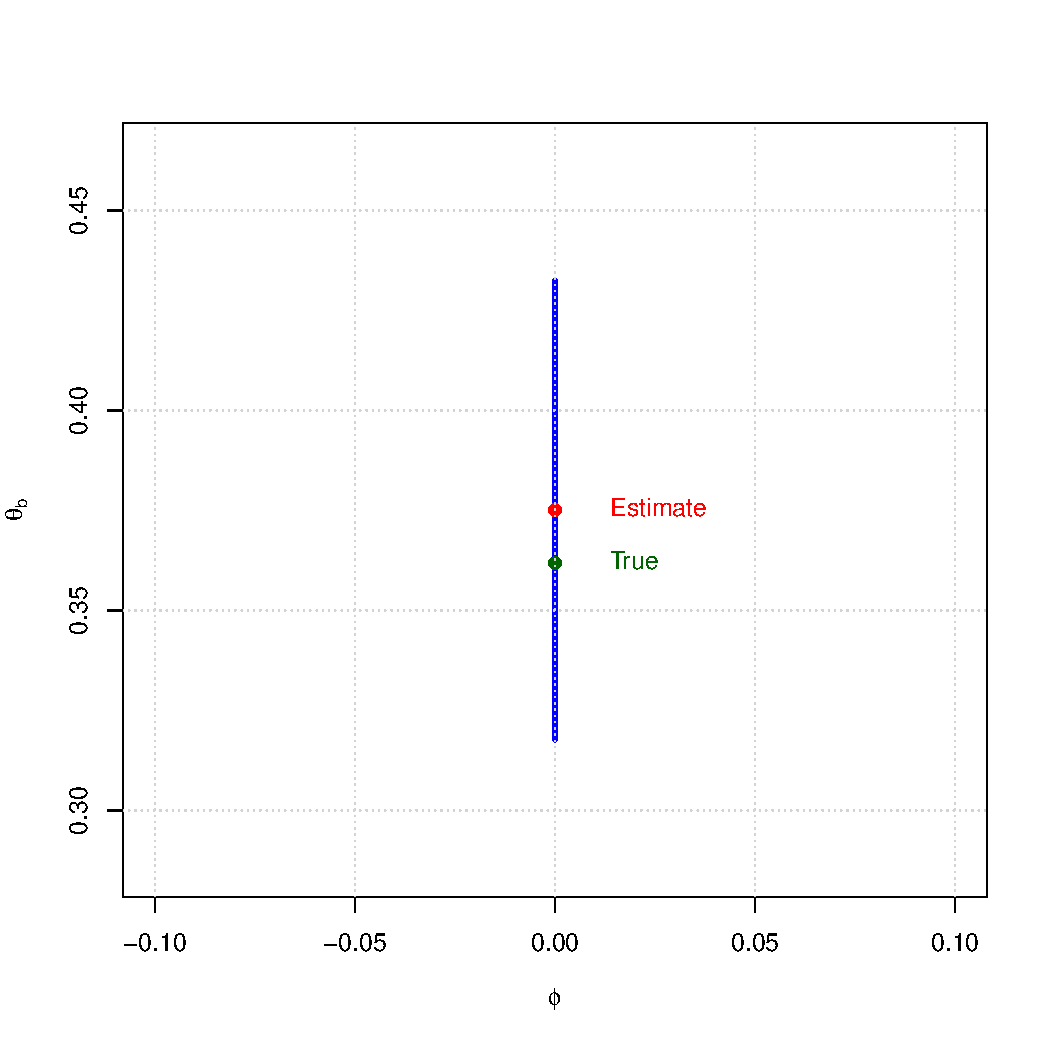
\includegraphics[width=\linewidth]{images/output/single_sim_ar_restricted.pdf}
        \caption{Confidence region for $\theta_b$ after restricting model}
    \end{subfigure}
    \hfill
    \begin{subfigure}{0.45\textwidth}
        \centering
        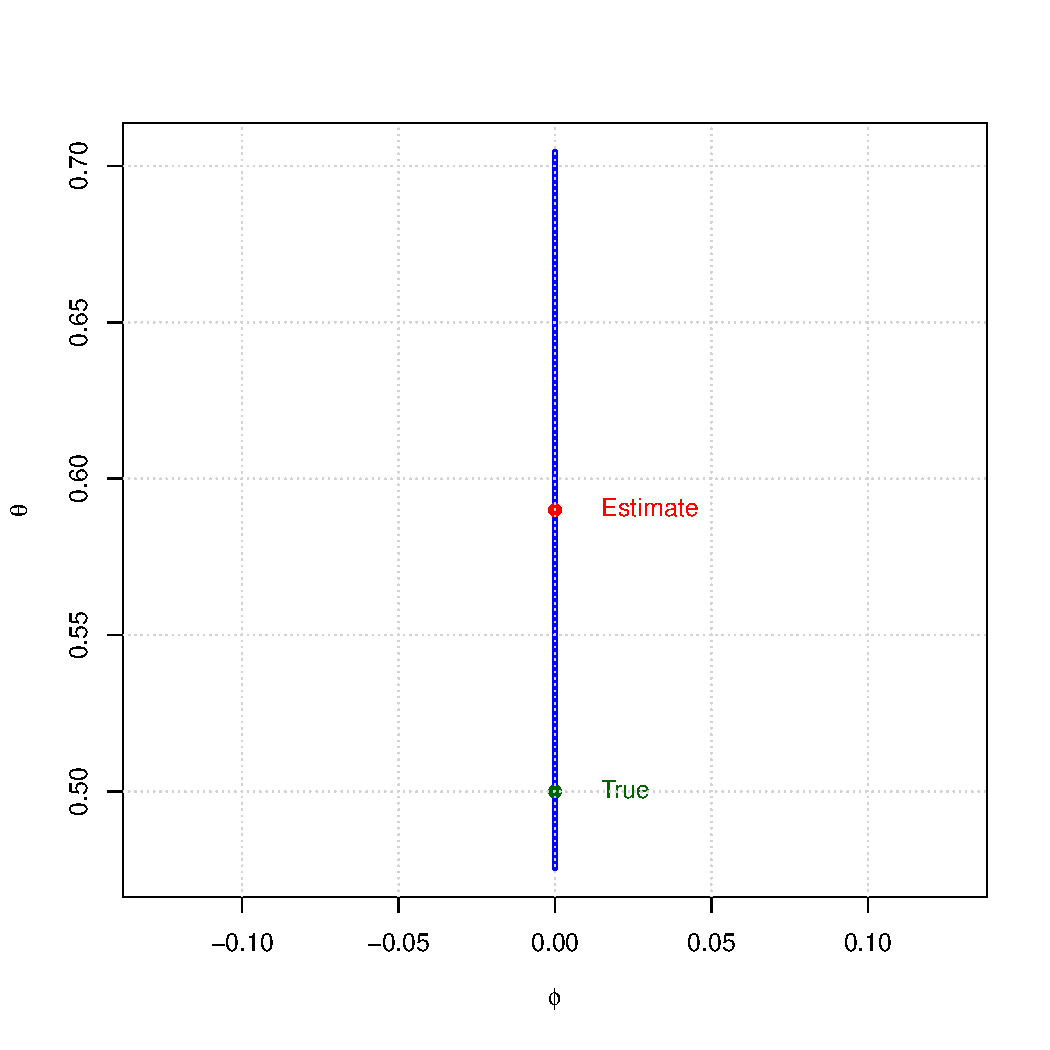
\includegraphics[width=\linewidth]{images/output/single_sim_ar_restricted_latent.pdf}
        \caption{Confidence Interval for $\theta$ after restricting model}
    \end{subfigure}

    % \vspace{0.5em}

    % % Row 2
    % \begin{subfigure}{0.45\textwidth}
    %     \centering
    %     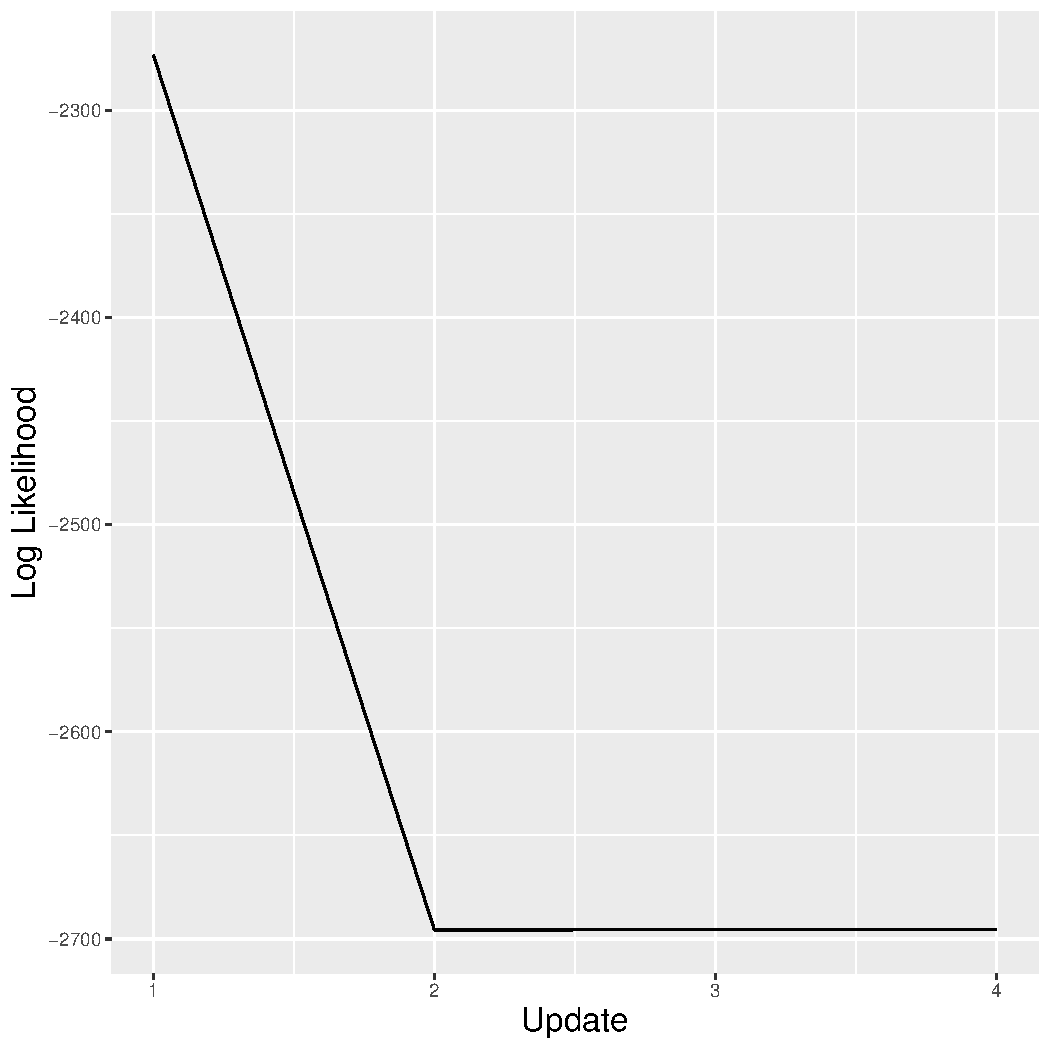
\includegraphics[width=\linewidth]{images/output/sim_mab_l2.pdf}
    %     \caption{Caption 3}
    % \end{subfigure}
    % \hfill
    % \begin{subfigure}{0.45\textwidth}
    %     \centering
    %     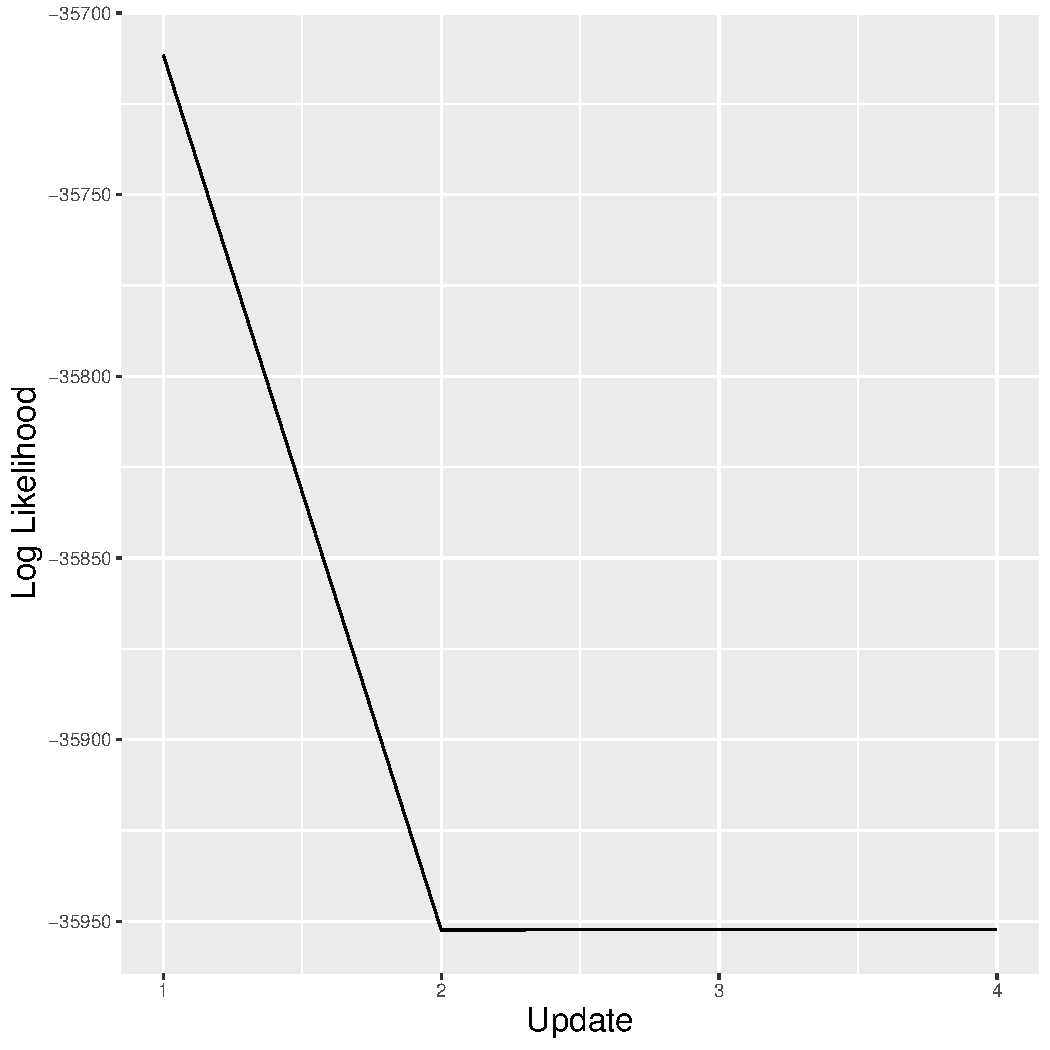
\includegraphics[width=\linewidth]{images/output/sim_mab_l.pdf}
    %     \caption{Caption 4}
    % \end{subfigure}

    \caption{Confidence regions for observable and latent moving average parameters after restricting REMARCS model with $\theta_b = 0$}
    \label{fig:conf_regions_observed_ar}
\end{figure}

Note that while the point estimate $\hat{\theta}$ doesn't change much, the range of the confidence interval for $\theta$ has shrunk with the decrease in degrees of freedom.

\subsubsection{Case: $\mathbf{w}$ is AR(1)}

We now look to the special case in which aggregate noise is an AR(1) process, which we recall can only occur if $\theta/\phi = \mathbb{E}(N^{-1})\sigma_\varepsilon^2/\sigma_\eta^2$. We select parameters for which this equality doesn't hold exactly, but is approximately true given the distribution of $N_t$:

\begin{table}[H]
\centering\begin{tabular}{lccccccccc}
\hline
$T$ & sims & $\phi$ & $\theta$ & $\sigma_\eta^2$ & $\sigma_\varepsilon^2$ & $\beta_0$ & $\beta_1$ & $\beta_2$ \\
1000 & 1 & 0.5 & 0.5 & 5.25 & 50 & 20 & -0.001 & 2 \\
\hline
\end{tabular}
\caption{Parameter values for simulated REMARCS model with latent AR(1) process }
\label{tab:param_values_mab}
\end{table}





\begin{figure}[H]
    \centering

    % Row 1
    \begin{subfigure}{0.45\textwidth}
        \centering
        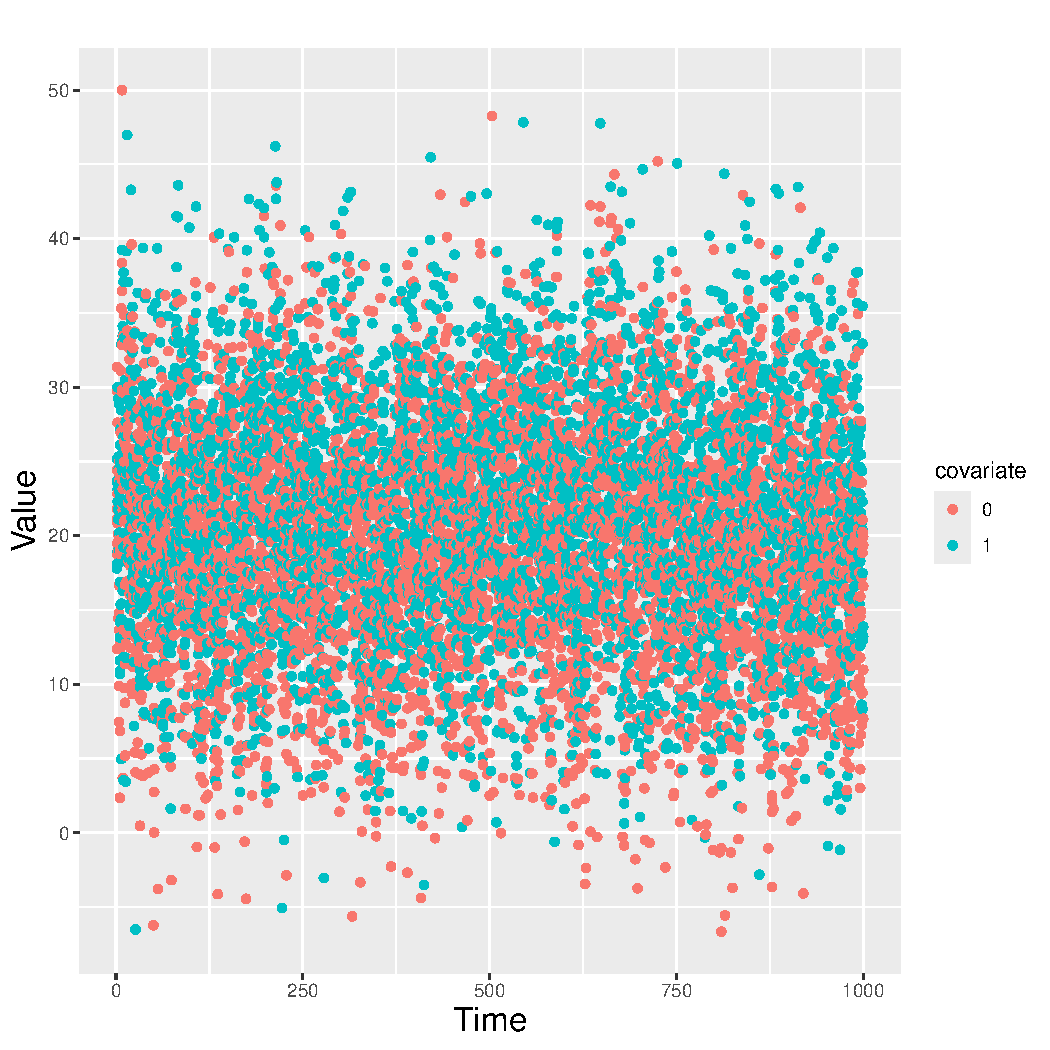
\includegraphics[width=\linewidth]{images/output/sim_mab_full.pdf}
        \caption{Observations}
    \end{subfigure}
    \hfill
    \begin{subfigure}{0.45\textwidth}
        \centering
        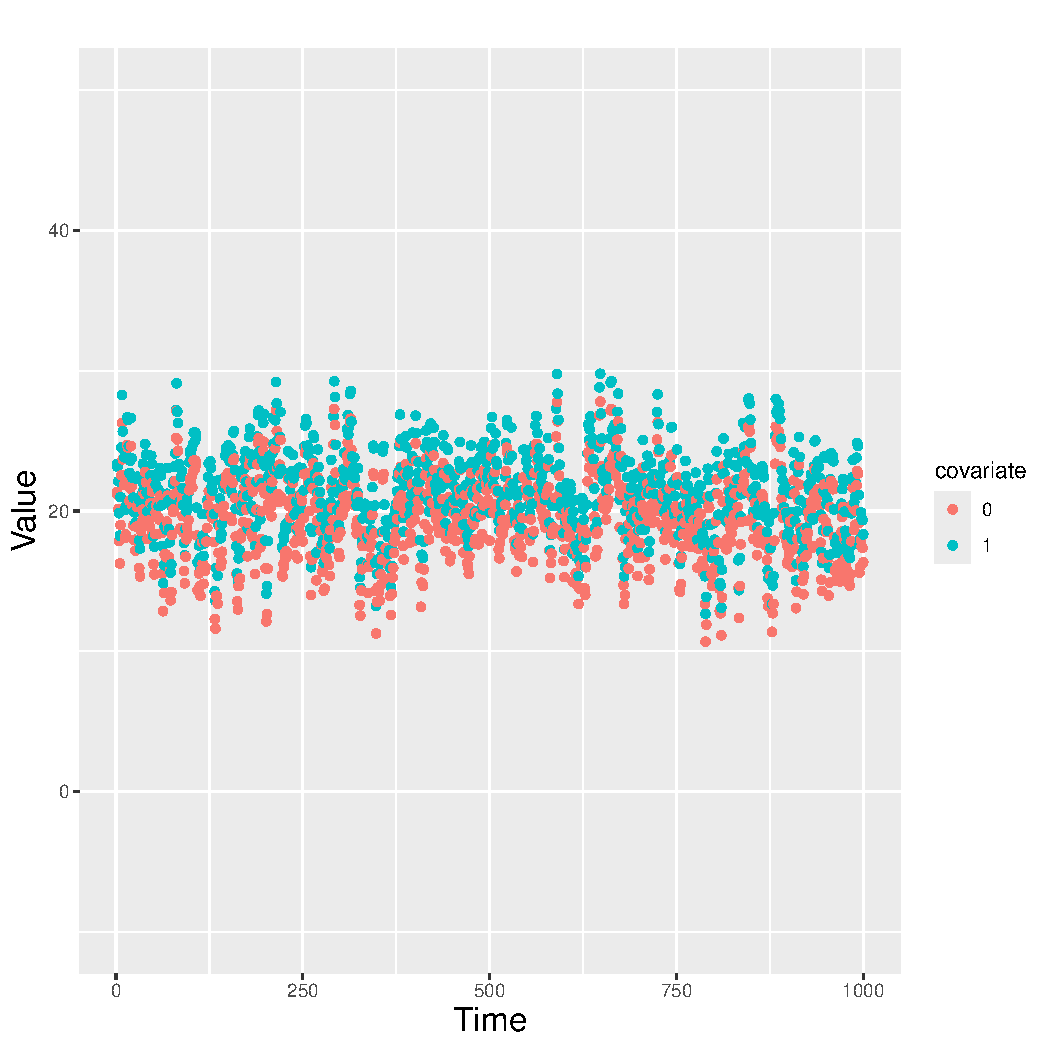
\includegraphics[width=\linewidth]{images/output/sim_mab_fitted.pdf}
        \caption{Fitted Values}
    \end{subfigure}

    % \vspace{0.5em}

    % % Row 2
    % \begin{subfigure}{0.45\textwidth}
    %     \centering
    %     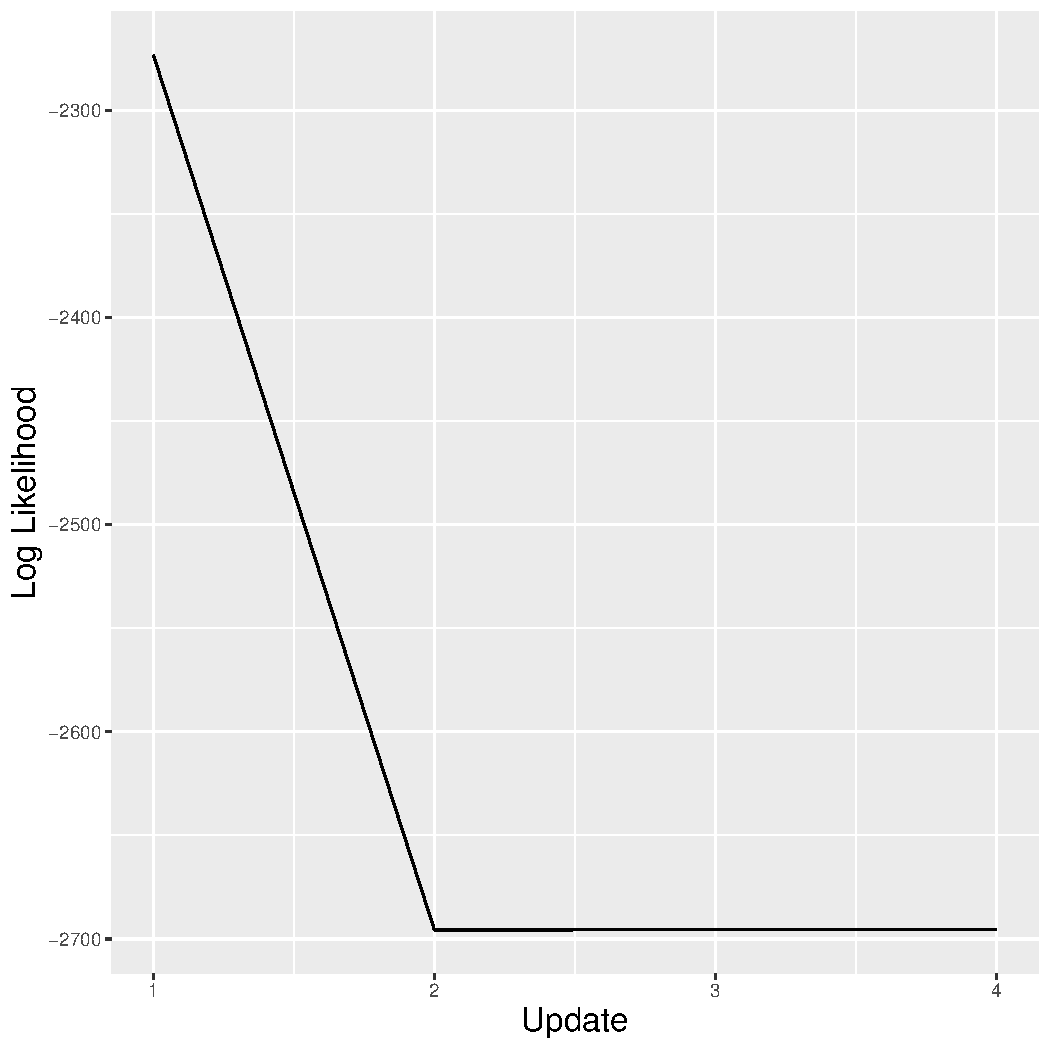
\includegraphics[width=\linewidth]{images/output/sim_mab_l2.pdf}
    %     \caption{Caption 3}
    % \end{subfigure}
    % \hfill
    % \begin{subfigure}{0.45\textwidth}
    %     \centering
    %     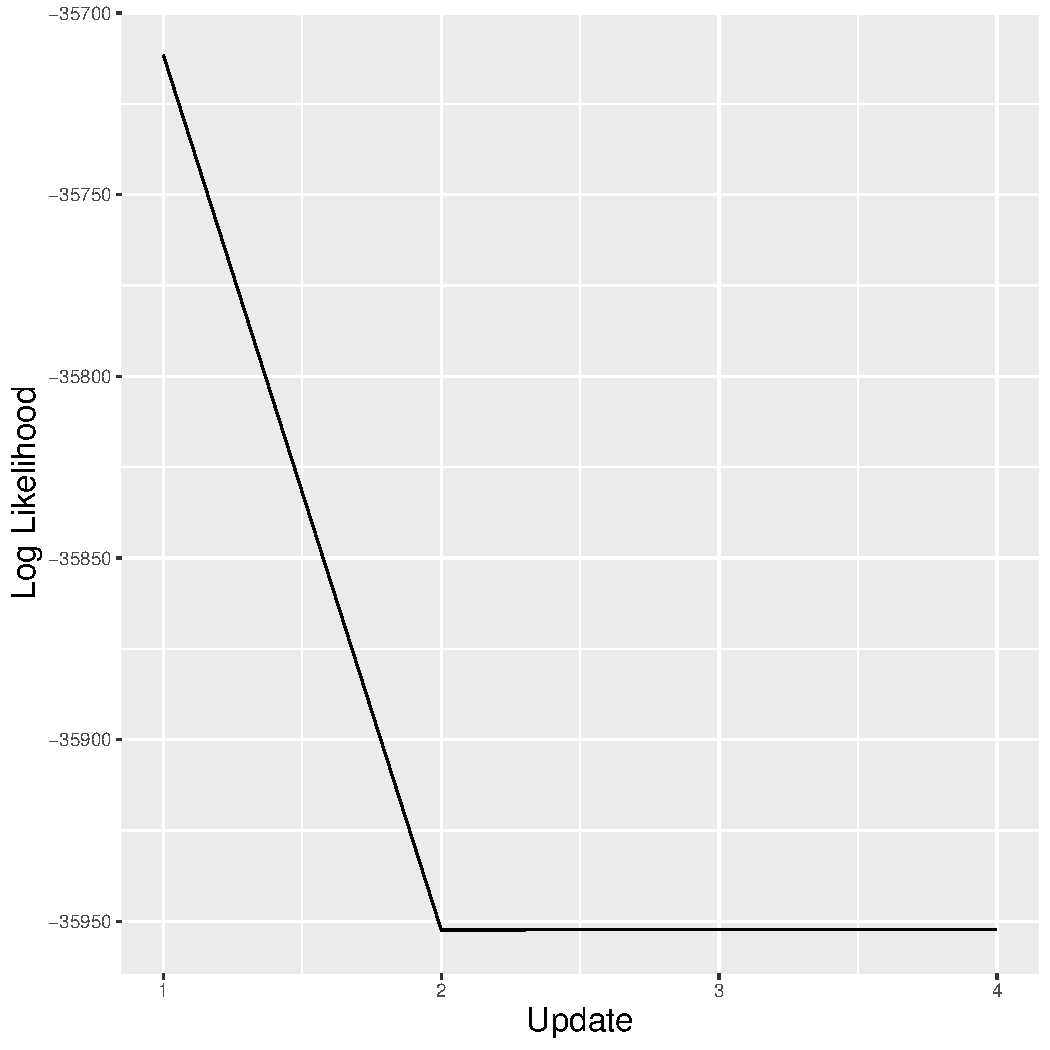
\includegraphics[width=\linewidth]{images/output/sim_mab_l.pdf}
    %     \caption{Caption 4}
    % \end{subfigure}

    \caption{Realization of a REMARCS Model in which the sum of the latent time series and aggregated cross-sectional noise is an AR(1) process}
    \label{fig:single_sim_mab}
\end{figure}

After fitting a REMARCS model to the data we obtain parameter estimates shown in Table \ref{tab:param_estimates_mab} and fitted values in Figure \ref{fig:single_sim_mab}. 

\begin{table}[H]
\centering\begin{tabular}{lccccccc}
\toprule
Parameter & $\beta_0$ & $\beta_1$ & $\beta_2$ & $\sigma_\varepsilon^2$ & $\phi$ & $\theta$ & $\sigma_\eta^2$ \\
\midrule
True Value & 20.0000 & -0.0010 & 2.0000 & 50.0000 & 0.5000 & 0.5000 & 5.2500 \\
\midrule
Initial estimate & 19.6845 & -0.0007 & 2.0362 & 61.4985 & 0.0000 & 0.0000 & 0.0000 \\
Final estimate & 19.7719 & -0.0008 & 1.9851 & 49.7772 & 0.4996 & 0.4962 & 5.1336 \\
\hline
\end{tabular}
\caption{Parameter estimates for REMARCS model with $\theta_b \approx 0$, before and after convergence}
\label{tab:param_estimates_mab}
\end{table}



Note that while the point estimate for $\theta$ given by Table \ref{tab:param_estimates_mab} is accurate, the confidence region thereof (Figure \ref{fig:sim_mab_unrestricted}) practically spans all of $(0,1)$, with which all that can be said is that $\theta$ is positive. 

\begin{figure}[H]
    \centering
    \begin{subfigure}{0.45\textwidth}
        \centering
        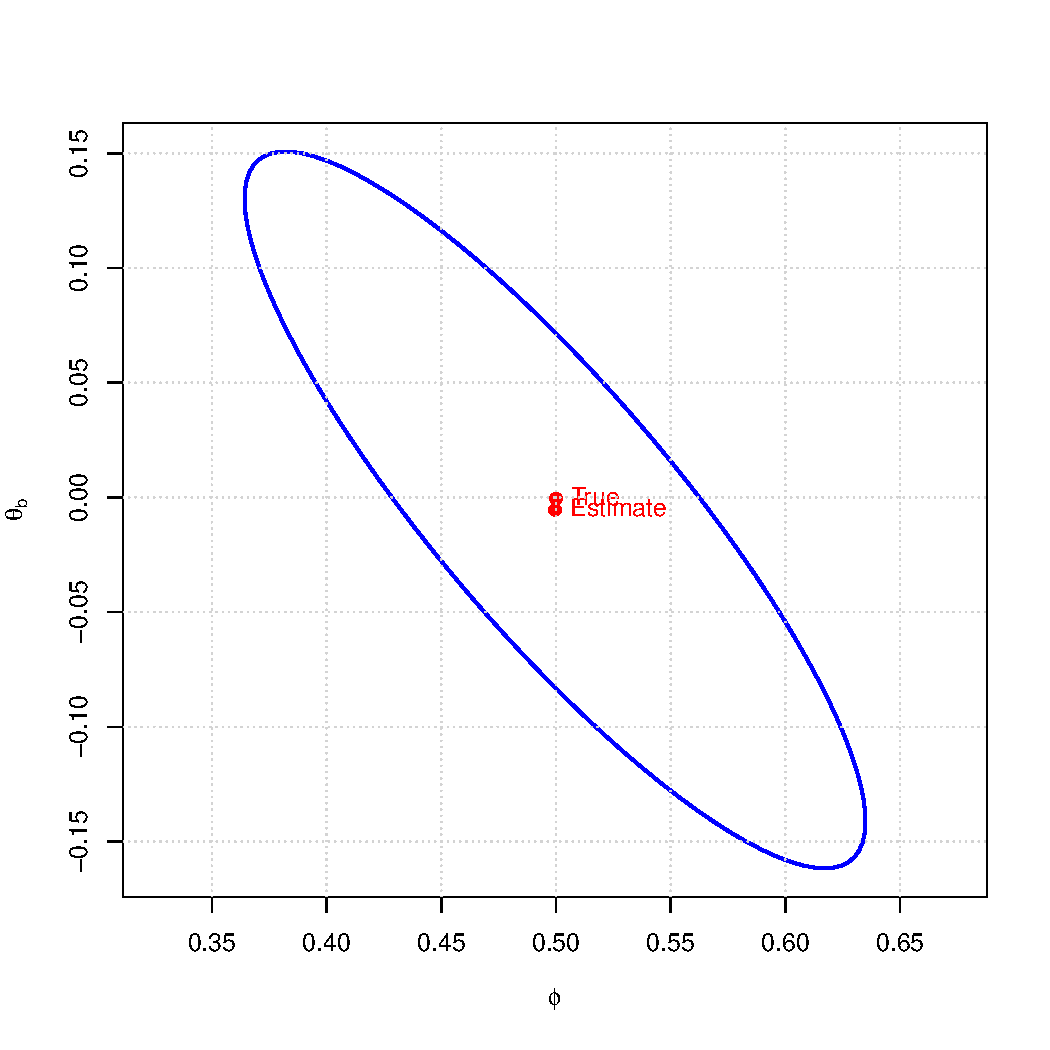
\includegraphics[width=\linewidth]{images/output/sim_mab_observed.pdf}
        \caption{Confidence region for $(\phi,\theta_b)$}
    \end{subfigure}
    \hfill
    \begin{subfigure}{0.45\textwidth}
        \centering
        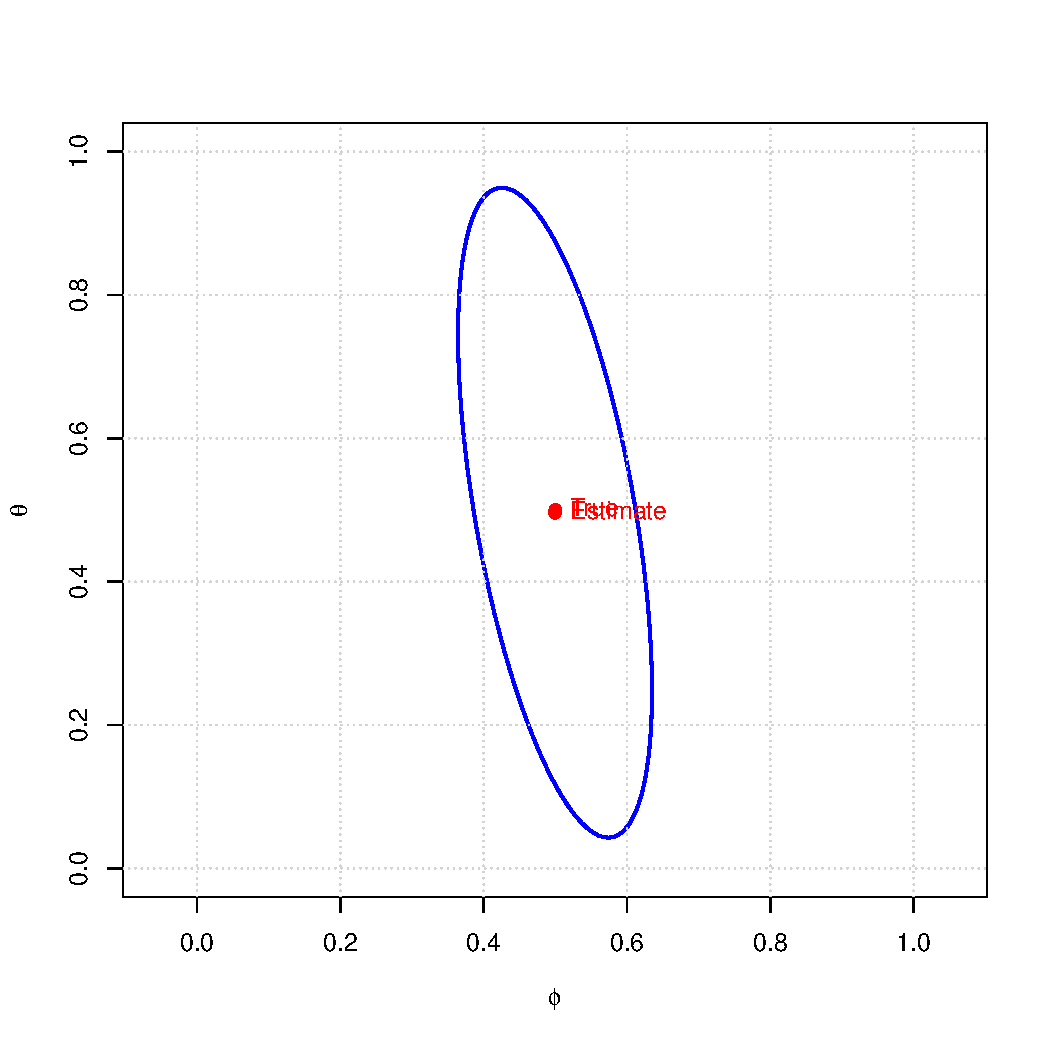
\includegraphics[width=\linewidth]{images/output/sim_mab_latent.pdf}
        \caption{Confidence region for $\phi,\theta$}
    \end{subfigure}
    \caption{Inference on ARMA parameters of REMARCS model in which $\theta_b = 0$ with restricted model}
    \label{fig:sim_mab_unrestricted}
\end{figure}
Note in the left panel of the same figure we see that the estimate for $\theta_b$ is insignificant, prompting us to refit $\mathbf{w}$ with an AR(1) model and use $H_{\theta_b}$ (Equation \ref{eq:H_thetab}) to construct a confidence region for $\hat{\theta}$, the products of which are shown in Figure \ref{fig:sim_mab_restricted}:

\begin{figure}[H]
    \centering
    \begin{subfigure}{0.45\textwidth}
        \centering
        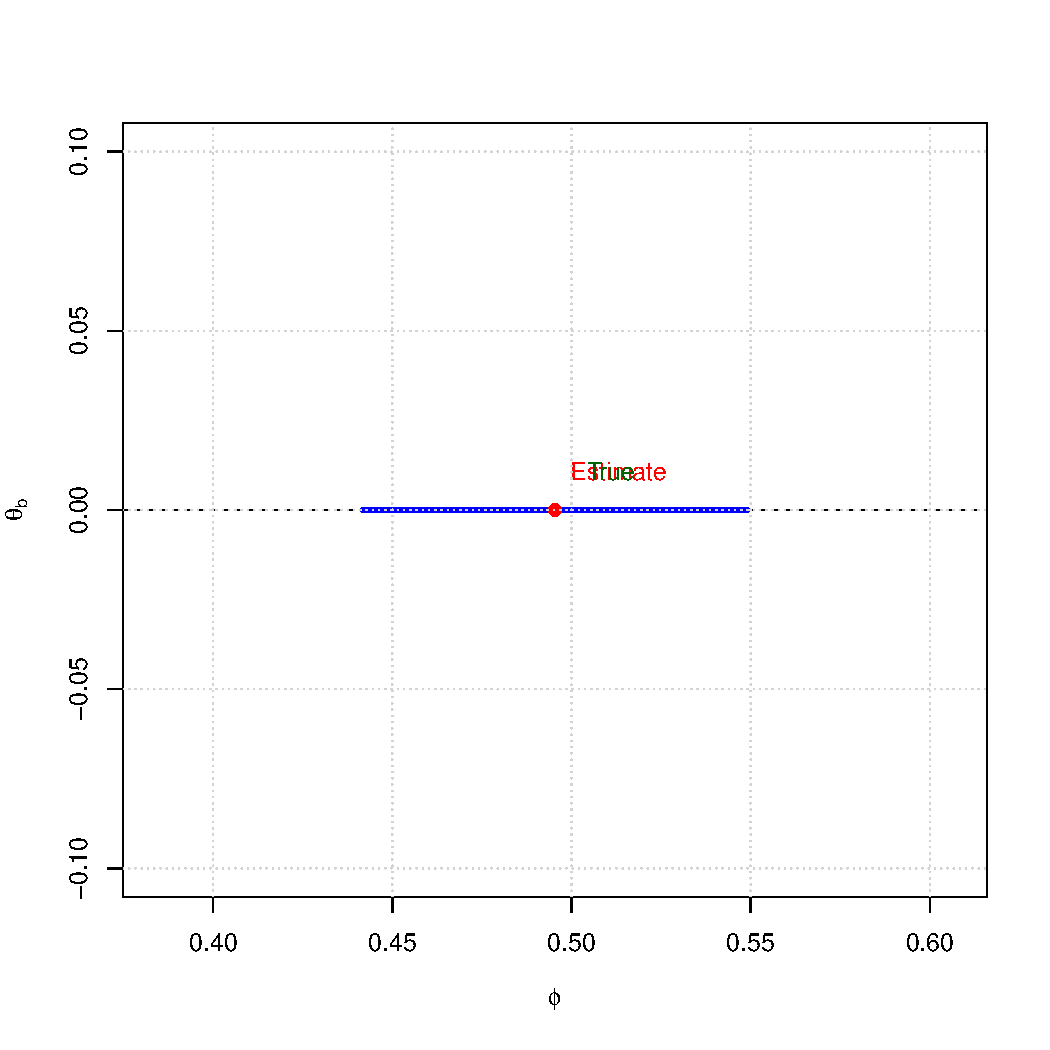
\includegraphics[width=\linewidth]{images/output/single_dim_mab_restricted.pdf}
        \caption{Confidence region for $(\phi,\theta_b)$}
    \end{subfigure}
    \hfill
    \begin{subfigure}{0.45\textwidth}
        \centering
        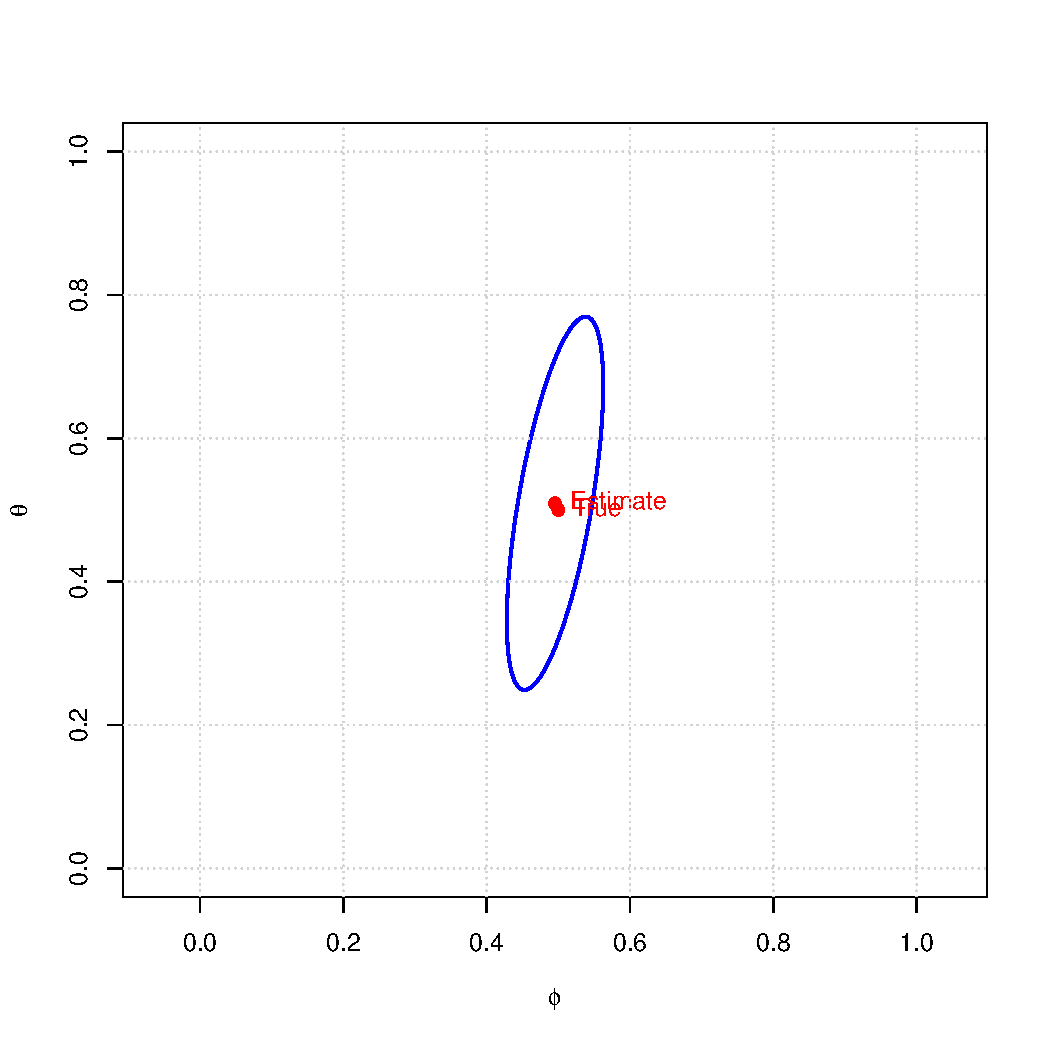
\includegraphics[width=\linewidth]{images/output/sim_mab_restricted.pdf}
        \caption{Confidence region for $\phi,\theta$}
    \end{subfigure}
    \caption{Inference on ARMA parameters of REMARCS model in which $\theta_b = 0$ with restricted model}
    \label{fig:sim_mab_restricted}
\end{figure}

We now obtain a confidence interval for $\theta$ markedly smaller than before. Another change of note is that the correlation between $\hat{\phi}$ and $\hat{\theta}$ has gone from negative to positive. This makes sense given that the ratio between the two now has an added restriction. 

Now that our algorithm has demonstrated promising results on simulated data, we observe how it performs on real RCS survey data.